\documentclass[runningheads,a4paper]{llncs}
\usepackage{standalone}

% Fix the nocite command in combination with the standalone package
\makeatletter
\def\@documentnocite#1{\@bsphack
  \@for\@citeb:=#1\do{%
    \edef\@citeb{\expandafter\@firstofone\@citeb}%
    \if@filesw\immediate\write\@auxout{\string\citation{\@citeb}}\fi
    \@ifundefined{b@\@citeb}{\G@refundefinedtrue
      \@latex@warning{Citation `\@citeb' undefined}}{}}%
  \@esphack}
\AtBeginDocument{\let\nocite\@documentnocite}
\makeatother

\input{"preamble.tex"}

%\makeatletter\@openrightfalse\makeatother 

\begin{document}
\mainmatter
\maketitle

\begin{abstract}
We introduce geometric pattern mining, the problem of finding recurring local structure in discrete, geometric matrices. It differs from existing pattern mining problems by identifying complex spatial relations between elements, resulting in arbitrarily shaped patterns. After we formalise this new type of pattern mining, we propose an approach to selecting a set of patterns using the Minimum Description Length principle. We demonstrate the potential of our approach by introducing Vouw, a heuristic algorithm for mining exact geometric patterns. We show that Vouw delivers high-quality results with a synthetic benchmark.
\end{abstract}


\documentclass{llncs}
\usepackage[utf8]{inputenc}
\usepackage{verbatim}
\usepackage{multicol}
\usepackage{llncsdoc}
\usepackage{amsmath}
\usepackage{amsfonts}
\usepackage{amssymb}
\usepackage{graphicx}
\usepackage{lmodern}
\usepackage{calc}
\usepackage{enumitem}
\usepackage{algpseudocode}
\usepackage{algorithm}
\usepackage{algorithmicx}

\algsetblockdefx[IfContinue]{IfContinue}{IfContinue}
{0}{0pt}
[0]{}
[1]{\textbf{if} #1 \textbf{continue}}

\algrenewcommand\algorithmicrequire{%
  \makebox[\widthof{\textbf{Output:}}][l]{\textbf{Input:}}}
  
 \algrenewcommand\algorithmicensure{%
  \textbf{Output:}}

\usepackage{color}
\usepackage{gnuplottex}
\usepackage{subcaption}
\usepackage{microtype}
\usepackage[normalem]{ulem}
\captionsetup{compatibility=false}
\usepackage{tikz}
\usetikzlibrary{trees,automata,positioning}
\usepackage{booktabs}
\usepackage{gnuplottex}
\usepackage{xparse}
\usepackage{epstopdf}
% For scaling gnuplottex
\ExplSyntaxOn
\DeclareExpandableDocumentCommand{\convertlen}{ O{cm} m }
 {
  \dim_to_unit:nn { #2 } { 1 #1 } cm
 }
\ExplSyntaxOff

%% For lattice figure
% Set the overall layout of the tree
\tikzstyle{level 1}=[level distance=3.0cm, sibling distance=0.6cm]
\tikzstyle{level 2}=[level distance=3.5cm, sibling distance=0.6cm]
\tikzstyle{level 3}=[level distance=3.5cm, sibling distance=0.6cm]

% Define styles for bags and leafs
\tikzstyle{l1} = [rectangle, text width=5em, text centered]
\tikzstyle{l2} = [rectangle, text width=5em, text centered]
\tikzstyle{l3} = [rectangle, text width=5em, text centered]

% only when using asmthm
%\newtheorem{definition}{Definition}
%\newtheorem{theorem}{Theorem}

\author{Micky Faas \and Matthijs van Leeuwen}
\title{VOUW: Geometric Pattern Mining using the MDL Principle}
\institute{Leiden Institute for Advances Computer Science}
\begin{document}

\section{Introduction}

Frequent pattern mining \cite{aggarwal2014fpm} is the well-known subfield of data mining that aims to find and extract recurring substructures from data, as a form of knowledge discovery. The generic concept of pattern mining has been instantiated for many different types of patterns, e.g., for item sets (in Boolean transaction data) and subgraphs (in graphs/networks). Little research, however, has been done on pattern mining for raster-based data, i.e., geometric matrices in which the row and column orders are fixed. The exception is geometric tiling \cite{gionis2004tiles,tatti2012stijl}, but that problem only considers tiles, i.e., rectangular-shaped patterns, in Boolean data.

\begin{figure}[b]
\centering
\begin{subfigure}[t]{0.35\textwidth}
\centering
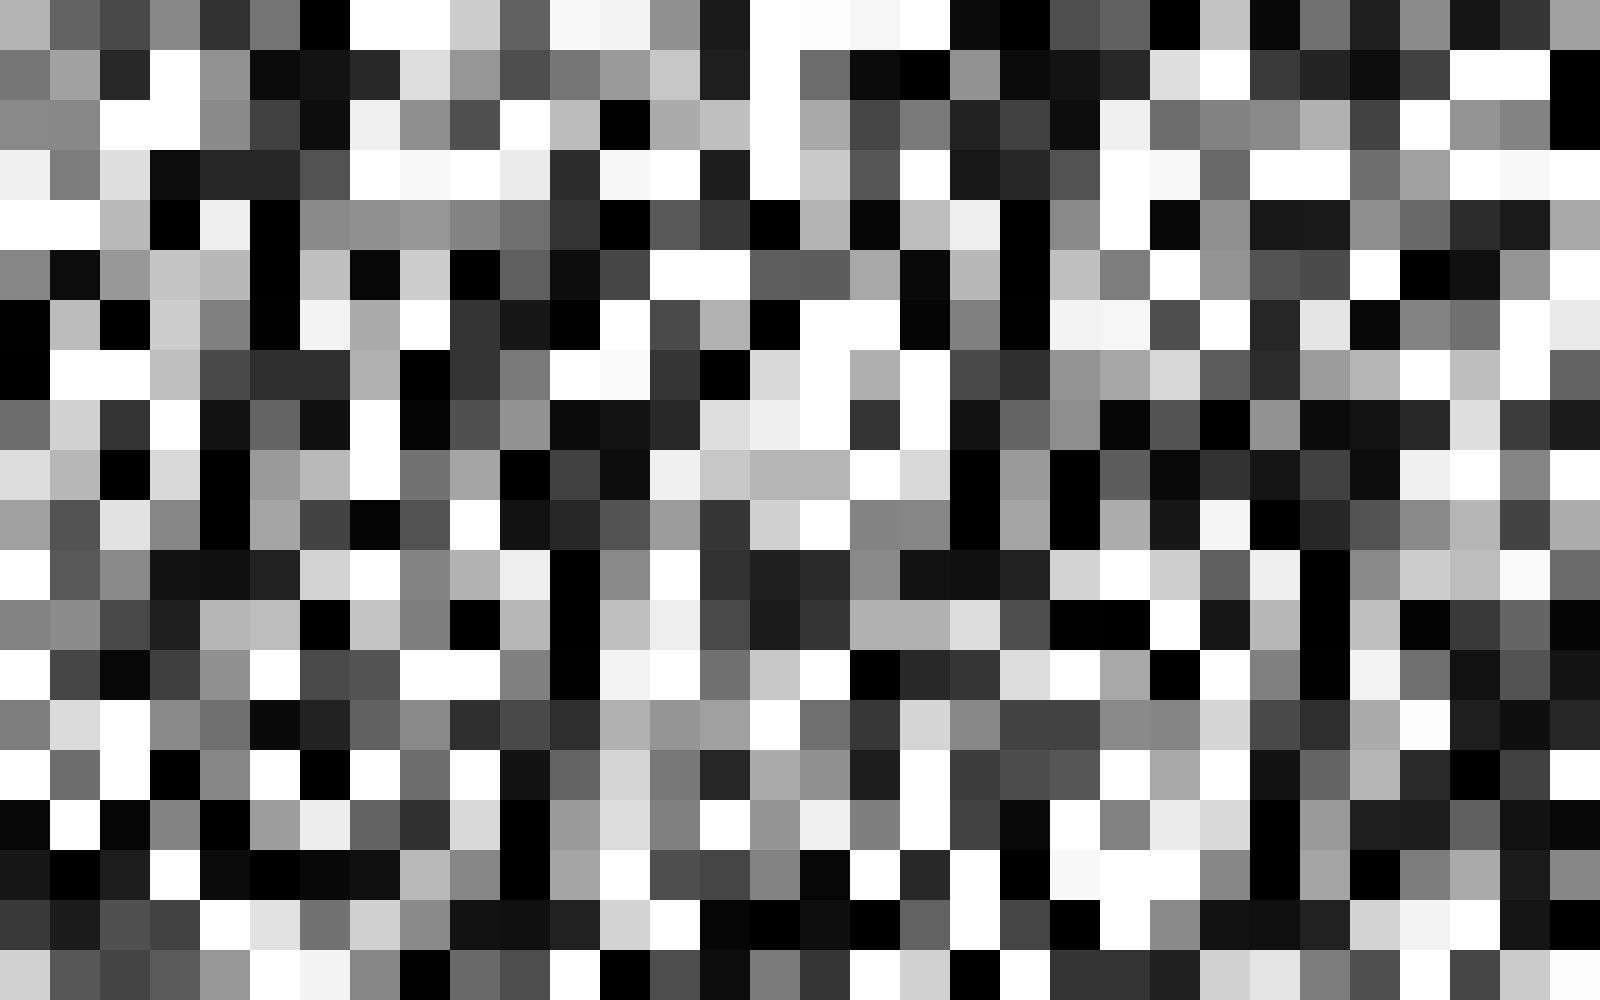
\includegraphics[scale=.25]{img/Garamond-I_cropped.png}
\caption{$32\times 24$ `geometric matrix'.}
\label{fig-example1a}
\end{subfigure}%
~
\begin{subfigure}[t]{0.21\textwidth}
\centering
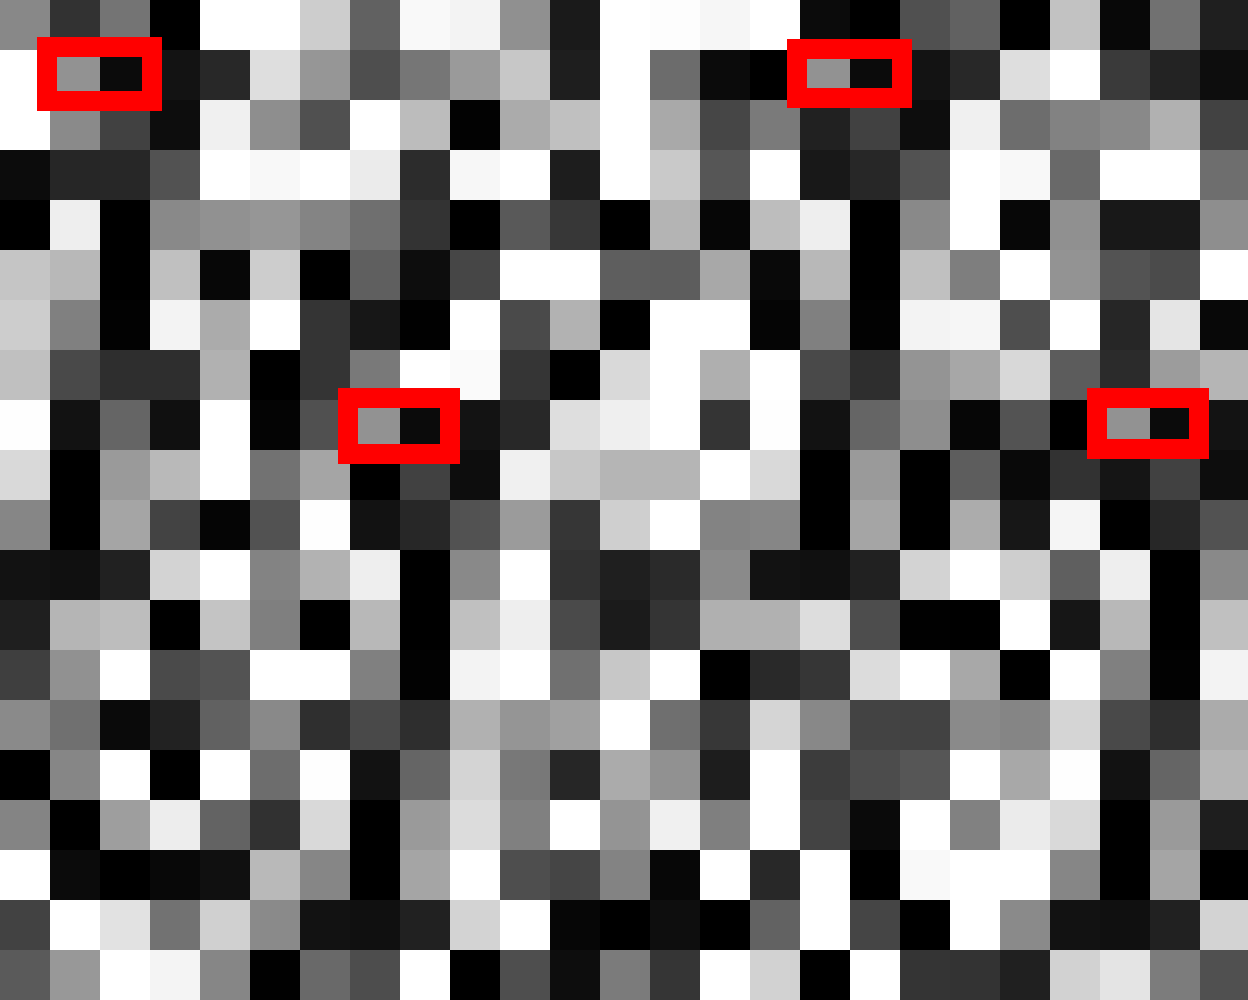
\includegraphics[scale=.25]{img/Garamond-I-highlight_cropped.png}
\caption{Pair $(146,11)$.}
\label{fig-example1b}
\end{subfigure}%
~
\begin{subfigure}[t]{0.37\textwidth}
\centering
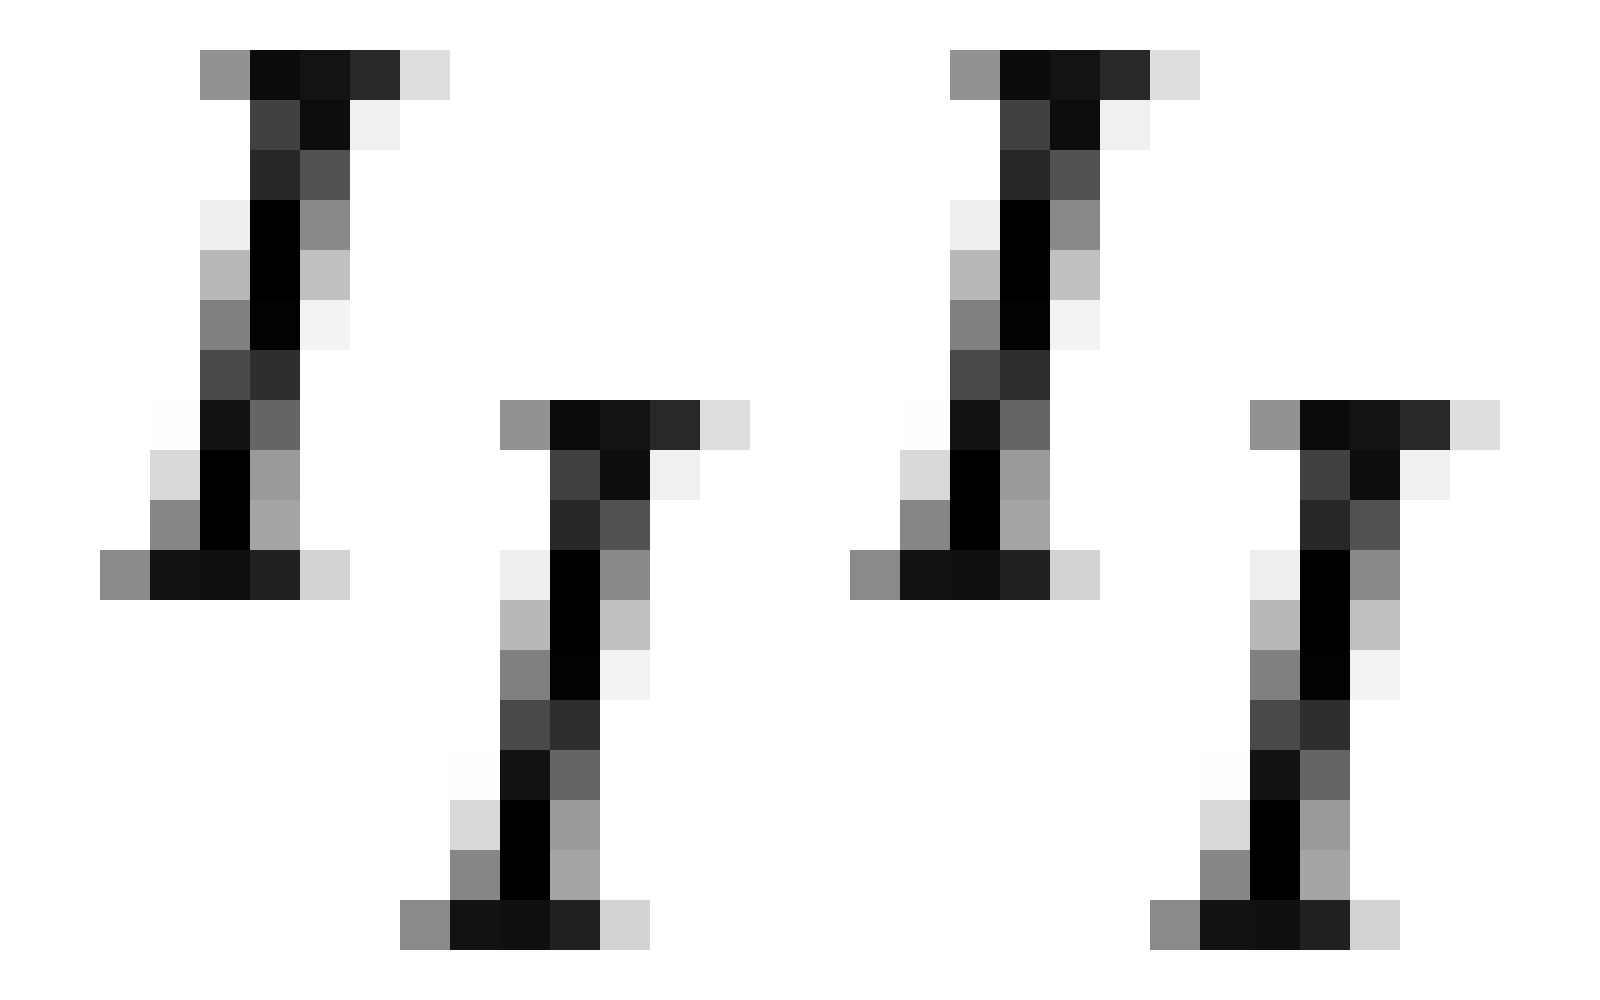
\includegraphics[scale=.25]{img/Garamond-I-clean_cropped.png}
\caption{Pattern `I' occurs four times.}
\label{fig-example1c}
\end{subfigure}%
\caption{Geometric pattern mining example. Each element is in $[0,255]$.}
\label{fig-example1}
\end{figure}  

In this paper we generalise this setting in two important ways. First, we consider geometric patterns \emph{of any shape} that are geometrically connected, i.e., it must be possible to reach any element from any other element in a pattern by only traversing elements in that pattern. Second, we consider \emph{discrete geometric data} with any number of possible values (which includes the Boolean case). We call the resulting problem \emph{geometric pattern mining}.

Figure~\ref{fig-example1} illustrates an example of geometric pattern mining.  Figure~\ref{fig-example1a} shows a $32 \times 24$ grayscale `geometric matrix', with each element in $[0,255]$, apparently filled with noise. If we take a closer look at all horizontal pairs of elements, however, we find that the pair $(146,11)$ is, amongst others, more prevalent than expected from `random noise' (Figure~\ref{fig-example1b}). If we would continue to try all combinations of elements that `stand out' from the background noise, we would eventually find four copies of the letter `I' set in 16 point Garamond Italic (Figure~\ref{fig-example1c}).

The 35 elements that make up a single `I' in the example form what we call a \emph{geometric pattern}. Since its four occurrences jointly cover a substantial part of the matrix, we could use this pattern to describe the matrix more succinctly than by 768 independent values. That is, we could describe it as the pattern `I' at locations $(5,4), (11,11), (20,3), (25,10)$ plus 628 independent values, hereby separating structure from accidental (noise) data. Since the latter description is shorter, we have compressed the data. At the same time we have learned something about the data, namely that it contains four I's. This suggests that we can use compression as a criterion to find patterns that describe the data.

\smallskip
\noindent \textbf{Approach and contributions}. Our first contribution is that we introduce and formally define \emph{geometric pattern mining}, i.e., the problem of finding recurring local structure in geometric, discrete matrices. Although we restrict the scope of this paper to two-dimensional data, the generic concept applies to higher dimensions. Potential applications include the analysis of satellite imagery, texture recognition, and (pattern-based) clustering.

We distinguish three types of geometric patterns: 1) \emph{exact} patterns, which must appear exactly identical in the data to match; 2) \emph{fault-tolerant} patterns, which may have noisy occurrences and are therefore better suited to noisy data; and 3) \emph{transformation-equivalent} patterns, which are identical after some transformation (such as mirror, inverse, rotate, etc.). Each consecutive type makes the problem more expressive and hence more complex. In this initial paper we therefore restrict the scope to the first, exact type.

As many geometric patterns can be found in a typical matrix, it is crucial to find a compact set of patterns that together describe the structure in the data well. We regard this as a model selection problem, where a model is defined by a set of patterns. Following our observation above, that geometric patterns can be used to compress the data, our second contribution is the formalisation of the model selection problem by using the \emph{Minimum Description Length (MDL) principle} \cite{rissanenmdl,grunwaldmdl}. Central to MDL is the notion that `learning' can be thought of as `finding regularity' and that regularity itself is a property of data that is exploited by \emph{compressing} said data. This matches very well with the goals of pattern mining, as a result of which the MDL principle has proven very successful for MDL-based pattern mining \cite{krimp,classy}.

Finally, our third contribution is Vouw, a heuristic algorithm for MDL-based geometric pattern mining that (1) finds compact yet descriptive sets of patterns, (2) requires no parameters, and (3) is tolerant to noise in the data (but not in the occurrences of the patterns). We empirically evaluate Vouw on synthetic data and demonstrate that it is able to accurately recover planted patterns.

\end{document}


\documentclass{llncs}
\usepackage[utf8]{inputenc}
\usepackage{verbatim}
\usepackage{multicol}
\usepackage{llncsdoc}
\usepackage{amsmath}
\usepackage{amsfonts}
\usepackage{amssymb}
\usepackage{graphicx}
\usepackage{lmodern}
\usepackage{calc}
\usepackage{enumitem}
\usepackage{algpseudocode}
\usepackage{algorithm}
\usepackage{algorithmicx}

\algsetblockdefx[IfContinue]{IfContinue}{IfContinue}
{0}{0pt}
[0]{}
[1]{\textbf{if} #1 \textbf{continue}}

\algrenewcommand\algorithmicrequire{%
  \makebox[\widthof{\textbf{Output:}}][l]{\textbf{Input:}}}
  
 \algrenewcommand\algorithmicensure{%
  \textbf{Output:}}

\usepackage{color}
\usepackage{gnuplottex}
\usepackage{subcaption}
\usepackage{microtype}
\usepackage[normalem]{ulem}
\captionsetup{compatibility=false}
\usepackage{tikz}
\usetikzlibrary{trees,automata,positioning}
\usepackage{booktabs}
\usepackage{gnuplottex}
\usepackage{xparse}
\usepackage{epstopdf}
% For scaling gnuplottex
\ExplSyntaxOn
\DeclareExpandableDocumentCommand{\convertlen}{ O{cm} m }
 {
  \dim_to_unit:nn { #2 } { 1 #1 } cm
 }
\ExplSyntaxOff

%% For lattice figure
% Set the overall layout of the tree
\tikzstyle{level 1}=[level distance=3.0cm, sibling distance=0.6cm]
\tikzstyle{level 2}=[level distance=3.5cm, sibling distance=0.6cm]
\tikzstyle{level 3}=[level distance=3.5cm, sibling distance=0.6cm]

% Define styles for bags and leafs
\tikzstyle{l1} = [rectangle, text width=5em, text centered]
\tikzstyle{l2} = [rectangle, text width=5em, text centered]
\tikzstyle{l3} = [rectangle, text width=5em, text centered]

% only when using asmthm
%\newtheorem{definition}{Definition}
%\newtheorem{theorem}{Theorem}

\author{Micky Faas \and Matthijs van Leeuwen}
\title{VOUW: Geometric Pattern Mining using the MDL Principle}
\institute{Leiden Institute for Advances Computer Science}
\begin{document}

\section{Related Work}

As the first pattern mining approach using the MDL principle, Krimp \cite{krimp} was one of the main sources of inspiration for this paper. Many papers on pattern-based modelling using MDL have appeared since, both improving search, e.g., Slim \cite{slim}, and extending to other problems, e.g., Classy \cite{classy} for rule-based classification.

The problem closest to ours is probably that of geometric tiling, as introduced by Gionis et al.\ \cite{gionis2004tiles} and later also combined with the MDL principle by Tatti and Vreeken \cite{tatti2012stijl}. Geometric tiling, however, is limited to Boolean data and rectangularly shaped patterns (tiles); we strongly relax both these limitations.

Campana et al. \cite{campana2010compression} also use matrix-like input data (textures) and develops a compression-based similarity measure. Their method, however, cannot be used for \emph{explanatory} data analysis as it relies on a generic image compression algorithm that is essentially a black box.

%Geometric pattern mining is different from graph mining, as a matrix is more rigid and each element has a fixed degree of connectedness/adjacency. It is also unrelated to linear algebra, other then using the term `matrix' and a comparable style of notation. 

\end{document}


%\documentclass{llncs}
\usepackage[utf8]{inputenc}
\usepackage{verbatim}
\usepackage{multicol}
\usepackage{llncsdoc}
\usepackage{amsmath}
\usepackage{amsfonts}
\usepackage{amssymb}
\usepackage{graphicx}
\usepackage{lmodern}
\usepackage{calc}
\usepackage{enumitem}
\usepackage{algpseudocode}
\usepackage{algorithm}
\usepackage{algorithmicx}

\algsetblockdefx[IfContinue]{IfContinue}{IfContinue}
{0}{0pt}
[0]{}
[1]{\textbf{if} #1 \textbf{continue}}

\algrenewcommand\algorithmicrequire{%
  \makebox[\widthof{\textbf{Output:}}][l]{\textbf{Input:}}}
  
 \algrenewcommand\algorithmicensure{%
  \textbf{Output:}}

\usepackage{color}
\usepackage{gnuplottex}
\usepackage{subcaption}
\usepackage{microtype}
\usepackage[normalem]{ulem}
\captionsetup{compatibility=false}
\usepackage{tikz}
\usetikzlibrary{trees,automata,positioning}
\usepackage{booktabs}
\usepackage{gnuplottex}
\usepackage{xparse}
\usepackage{epstopdf}
% For scaling gnuplottex
\ExplSyntaxOn
\DeclareExpandableDocumentCommand{\convertlen}{ O{cm} m }
 {
  \dim_to_unit:nn { #2 } { 1 #1 } cm
 }
\ExplSyntaxOff

%% For lattice figure
% Set the overall layout of the tree
\tikzstyle{level 1}=[level distance=3.0cm, sibling distance=0.6cm]
\tikzstyle{level 2}=[level distance=3.5cm, sibling distance=0.6cm]
\tikzstyle{level 3}=[level distance=3.5cm, sibling distance=0.6cm]

% Define styles for bags and leafs
\tikzstyle{l1} = [rectangle, text width=5em, text centered]
\tikzstyle{l2} = [rectangle, text width=5em, text centered]
\tikzstyle{l3} = [rectangle, text width=5em, text centered]

% only when using asmthm
%\newtheorem{definition}{Definition}
%\newtheorem{theorem}{Theorem}

\author{Micky Faas \and Matthijs van Leeuwen}
\title{VOUW: Geometric Pattern Mining using the MDL Principle}
\institute{Leiden Institute for Advances Computer Science}
\begin{document}

\section{Preliminaries}

\subsection{Data Mining Through Compression}

In the previous subsection we have discussed that the input matrix can be expressed in terms of patterns and instances, and that some combinations are more favourable than others. We need a way to quantize the quality of a description and we do this according to the MDL-principle. 

The Minimum Description Length Principle:
\begin{itemize}
\item Is a practical realization of Kolmogorov-complexity, which in itself is shown to be incomputable
\item Has multiple variants; we use the `crude' or two-part MDL equation
\item Is an optimization problem that tries to minimize the total length of the description of the input data
\item It can be shown that the most concise (but loss-less) description of the original data reveals the most information about the data
\item Finding a minimal loss-less description can be thought of as \emph{compression}, hence `datamining by compression'
\item This minimization problem usually has a huge search space and therefore most approaches use a greedy heuristic
\end{itemize}

Two-part MDL splits the description into the \emph{model} and the \emph{data given the model}. Minimizing the sum of their lengths prevents over- and underfitting. \emph{(Explain these terms in the context of our problem)}

\subsubsection{Priors and Encoding}

Apart from finding or approaching the optimal minimal description, the greatest challenge in MDL-based algorithms lies in the fact that we have to devise some kind of encoding scheme to compress the data. We must make this encoding scheme in such way that it can be decoded without loss of information.
\begin{itemize}
\item We will not actually encode the data each time, but rather just compute the length if it were encoded
\item There are multiple ways (\emph{priors}) of assigning code lengths to symbols according to their probability of occurring. \begin{itemize}
\item If we know the total number of symbols and the distribution is uniform, we use $-\log(p)$. This is the optimal code length accordig to Shannon's entropy. 
\item For integers on an unknown domain there is the Universal Prior for integers. 
\item Lastly, we use prequential-plugin code if we do not know the distribution in advance, but want to approach the uniform distribution for large sets of symbols.
\end{itemize}
\end{itemize}


\end{document}


\documentclass{llncs}
\usepackage[utf8]{inputenc}
\usepackage{verbatim}
\usepackage{multicol}
\usepackage{llncsdoc}
\usepackage{amsmath}
\usepackage{amsfonts}
\usepackage{amssymb}
\usepackage{graphicx}
\usepackage{lmodern}
\usepackage{calc}
\usepackage{enumitem}
\usepackage{algpseudocode}
\usepackage{algorithm}
\usepackage{algorithmicx}

\algsetblockdefx[IfContinue]{IfContinue}{IfContinue}
{0}{0pt}
[0]{}
[1]{\textbf{if} #1 \textbf{continue}}

\algrenewcommand\algorithmicrequire{%
  \makebox[\widthof{\textbf{Output:}}][l]{\textbf{Input:}}}
  
 \algrenewcommand\algorithmicensure{%
  \textbf{Output:}}

\usepackage{color}
\usepackage{gnuplottex}
\usepackage{subcaption}
\usepackage{microtype}
\usepackage[normalem]{ulem}
\captionsetup{compatibility=false}
\usepackage{tikz}
\usetikzlibrary{trees,automata,positioning}
\usepackage{booktabs}
\usepackage{gnuplottex}
\usepackage{xparse}
\usepackage{epstopdf}
% For scaling gnuplottex
\ExplSyntaxOn
\DeclareExpandableDocumentCommand{\convertlen}{ O{cm} m }
 {
  \dim_to_unit:nn { #2 } { 1 #1 } cm
 }
\ExplSyntaxOff

%% For lattice figure
% Set the overall layout of the tree
\tikzstyle{level 1}=[level distance=3.0cm, sibling distance=0.6cm]
\tikzstyle{level 2}=[level distance=3.5cm, sibling distance=0.6cm]
\tikzstyle{level 3}=[level distance=3.5cm, sibling distance=0.6cm]

% Define styles for bags and leafs
\tikzstyle{l1} = [rectangle, text width=5em, text centered]
\tikzstyle{l2} = [rectangle, text width=5em, text centered]
\tikzstyle{l3} = [rectangle, text width=5em, text centered]

% only when using asmthm
%\newtheorem{definition}{Definition}
%\newtheorem{theorem}{Theorem}

\author{Micky Faas \and Matthijs van Leeuwen}
\title{VOUW: Geometric Pattern Mining using the MDL Principle}
\institute{Leiden Institute for Advances Computer Science}
\begin{document}

\section{Theoretical Framework}

%\subsection{On Patterns and Matrices}

%In this subsection we will introduce a method for describing and decomposing tabular or matrix-like data. It is this concise notation that allows us to reason about what one can and cannot expect to find from a set of data and what this data could look like. In later subsections we will use these tools to gradually connect to the MDL principle and finally to a practical search algorithm.

We define geometric pattern mining on bounded, discrete and two-dimensional raster-based data. We represent this data as an $M\times N$ matrix $A$ whose rows and columns are finite and in a fixed ordering (i.e. reordering rows and columns semantically alters the matrix). For elements $a_{i,j}$, where row $i$ is on $[0;N)$ and column $j$ is on $[0;M)$, holds that $a_{i,j} \in S$, the finite set of symbols occurring in $A$. %We will denote $A$ as a matrix because of the convenience of the linear algebra notation\footnote{In any practical application however, $A$ will not represent a system of linear equations but rather hold some form of sampled data that can be placed on a grid.}

\begin{figure}

\small
$$
A =
\begin{bmatrix}
1 & \cdot & \cdot & \cdot & 1 & 1 &  \\[-.2em]
\cdot & 1 & \cdot & \cdot & \cdot & \cdot &  \\[-.2em]
1 & \cdot & \cdot & \cdot & 1 & \cdot &  \\[-.2em]
\cdot & 1 & \cdot & \cdot & \cdot & 1 &  \\[-.2em]
1 & 1 & 1 & 1 & \cdot & \cdot &  \\
\end{bmatrix}\!\!, \
I = 
\begin{bmatrix}
X & \cdot & \cdot & \cdot & Y & \cdot & \\[-.2em]
\cdot & \cdot & \cdot & \cdot & \cdot & \cdot &  \\[-.2em]
X & \cdot & \cdot & \cdot & X & \cdot &  \\[-.2em]
\cdot & \cdot & \cdot & \cdot & \cdot & \cdot &  \\[-.2em]
Y & \cdot & Y & \cdot & \cdot & \cdot &  \\[-.2em]
\end{bmatrix}\!\!, \
H = \left\{
X =
\begin{bmatrix}
1 & \cdot \\[-.2em]
\cdot & 1
\end{bmatrix}\!\!,
Y =
\begin{bmatrix}
1 & 1
\end{bmatrix}\right\}
$$
\caption{Example decomposition of $A$ into instantiation $I$ and patterns $X,Y$.}

\label{example1}
\end{figure}

According to MDL, the shortest (optimal) description of $A$ reveals all structure of $A$ in the most succinct way possible and we approximate this optimal description through the compression of the original data. This optimal description $A'$ is only optimal if we can unambiguously reconstruct $A$ from it and nothing more --- the compression is both minimal and lossless. Intuitively compression means defining $A$ using as few building blocks as possible. We illustrate this in Figure \ref{example1}. Given the matrix $A$ we decompose it in patterns, denoted $X$ and $Y$. The set of all these patterns is the \textbf{model} of a $A$, denoted $H_A$. In order to reconstruct $A$ from this model, we alse need a mapping from the $H_A$ back to $A$. This mapping represents in what MDL calls the \textbf{the data given the model $H_A$}. In this context we think of it as `instructions' of how to reconstruct $A$. Let us call the set of all instructions required to rebuild $A$ from $H_A$ the \textbf{instantiation} of $H_A$. It is denoted by ${I}_A$ in the example.  The result is a notation that allows us to express matrix $A$ as if decomposed into sets of local and global spatial information, which we will now describe in more detail.

% Notice how $I_A$ essentially tells us where in $A$ each pattern from $H_A$ was originally located.

%We call a specific set of patterns $H\in \mathcal{H}_A$ a \textbf{point hypothesis} and analogously a specific instantiation is denoted ${I} \in \mathcal{I}_A$. Formally, a complete description $A'$ of $A$ is a combination of some $H$ and ${I}$ such that ${I}$ is a 1-to-1 mapping from $H_A$ to $A$. In the next subsections we will formalize these concepts by starting bottom-up with patterns and instances up to models, instantiation matrices and their link with MDL. After this we will discuss how we propose to find a good description of $A$ by means of the VOUW algorithm.


\subsection{Patterns and Instances}
\noindent $\triangleright$ \emph{We define a \textbf{pattern} as a $M_X\times N_X$ submatrix $X$ of the original matrix $A$. Elements of this submatrix may be $\cdot$, the empty element, which gives us the ability to cut-out any irregular-shaped part of $A$. We additionally require the elements of $X$ to be adjacent (horizontal, vertical or diagonal) to at least one non-empty element and that no rows and columns are empty.}
%While this limits the amount of possible patterns somewhat, it will later on also reduce the computational effort dramatically.
%We will now define a pattern to be the smallest submatrix to completely contain all elements of $X$.

%\begin{definition}
%A \textbf{pattern} $X$ is a $M_X\times N_X$ submatrix of $A$ where any non-empty element may %optionally be replaced by $\cdot$ such that:
%\begin{itemize}
%\item Any non-empty element in $X$ is adjacent (horizontal, vertical or diagonal) to at least one other non-%empty element.
%\item The first and last rows and columns contain at least one non-empty element.
%\end{itemize}
%\end{definition}
\smallskip

From this definition, the dimensions $M_X\times N_X$ give the smallest rectangle around $X$ (the \emph{bounding box)}. We also define the cardinality $|X|$ of $X$ as the number of non-empty elements. We call a pattern $X$ with $|X|=1$ a \textbf{singleton pattern}, i.e. a pattern containing exactly one element of $A$. %\footnote{We will often slightly abuse notation by using single-index elements or using set notation for any matrix. For instance, when we write $x_i \in X$, we mean that $x_i$ is the $i$-th non-empty element in $X$ with $1\leq i \leq |X|$. By convention we will always use row-major ordering in these cases.}

Each pattern contains a special \textbf{pivot} element: %
%\begin{definition}
$pivot(X)$ is the first non-empty element of $X$. % in the first non-empty column of the first (non-empty) row of $X$.
%\end{definition}
\noindent
A pivot can be thought of as a fixed point in $X$ which we can use to position its elements in relation to $A$. This translation, or \textbf{offset}, is a tuple ${q}=(i,j)$ that is on the same domain as an index in $A$. We realize this translation by placing all elements of $X$ on an empty $M\times X$ size matrix in such that the pivot element is at $(i,j)$. We formalize this in the \textbf{instantiation operator} $\otimes$:

\smallskip
\noindent $\triangleright$
%\begin{definition}
%In the context of an $M\times N$ matrix $A$,
\emph{We define the \textbf{instance} $X \otimes {(i,j)}$ as the $M\times N$ matrix containing all elements of $X$ such that $\mathrm{pivot}(X)$ is at index $(i,j)$ and the distances between all elements are preserved. The resulting matrix contains no additional non-empty elements. } %
%\end{definition}
\smallskip

%So according to this definition $\otimes$ adds `padding' around the elements of a pattern to align its pivot to a certain offset $(i,j)$. 
Obviously this does not yield a valid result for an arbitrary offset $(i,j)$. We want to limit ourselves to the space of pattern instances that are actually valid in relation to matrix $A$. Therefore two simple constraints are needed: (1) an instance must be \textbf{well-defined}: \emph{placing $\mathrm{pivot}(X)$ is at index $(i,j)$ results in an instance that contains all elements of $X$, and (2) elements of instances cannot overlap, meaning each element of $A$ should be described at most once.} This allows for a description that is both unambiguous and minimal.

\smallskip
%\begin{definition}
\noindent $\triangleright$
\emph{Two pattern instances $X \otimes {q}$ and $Y \otimes {r}$, with ${q} \neq {r}$ are \textbf{non-overlapping} if $|(X \otimes {q}) + (Y \otimes {r})| = |X|+|Y|$.}
%\end{definition}
\smallskip

From here on we will use the same letter in lower case to denote an arbitrary instance of a pattern, e.g. $x = X \otimes {q}$ when the exact value of ${q}$ is unimportant.%

We briefly introduced the instantiation $I$ as a set of `instructions' of where instances of each pattern should be positioned in order to obtain $A$. As Figure \ref{example1} suggests, this mapping has the shape of an $M\times N$ matrix.

\smallskip
%\begin{definition}
\noindent $\triangleright$
\emph{Given the set of patterns $H$, the \textbf{instantiation (matrix)} ${I}$ is an incomplete $M\times N$ matrix such that ${I}_{i,j} \in H \cup \{\cdot\}$ for all $(i,j)$. For all non-empty elements ${I}_{i,j}$ it holds that ${I}_{i,j} \otimes (i,j)$ is a non-overlapping instance of ${I}_{i,j}$ in $A$.}
%\end{definition}
\smallskip

The above definition creates the interesting proposition that the offset to each instance is unique. We provide a sketch proof in Appendix \ref{appendix_a} in \cite{archive}.
%Given that a pattern's pivot is placed exactly at one offset and that instances must be non-overlapping, makes this indeed believable. Later when we inductively define the set $\mathcal{I}$ of all instantiation matrices, this will be shown to be true more formally. 

%%
%% Removing this for now...
\begin{comment}
\subsection{Geometries}

In the previous subsections we silently omitted an important constraint in instantiating patterns. An instance has only meaning in the context of matrix $A$ if their respective elements match. In order words, if an instance $X \otimes (i,j)$ has all its non-empty elements identical to the corresponding indices in $A$, this means that pattern $X$ matches $A$ in $(i,j)$. In this case the match is exact, formally
\begin{definition}
The instance ${x}=X \otimes {q}$ is an \textbf{exact match on $A$} if for all non-empty ${x}_{i,j} \in {x}$ it holds that ${x}_{i,j} = a_{i,j}$.
\end{definition}

While this form of straightforward matching can be desirable in some cases, it may lead to a bloated model in others. Take the example from Figure \ref{example3} that lists matrix $A$ and four patterns. Pattern $W$ is obviously an exact match to five of the six elements of $A$. Pattern $X$, while not an exact match, is also a good candidate to describe $A$ although it is multiplied by a constant factor of two. Pattern $Y$ is a near-exact match: only one element is off - this could be due to noise for example. Pattern $Z$ is no match for the values in $A$, but notice that it is identical in structure to the other patterns: it places as many values at the same indices. 

\begin{figure}
\tiny
$$
\left.
A =
\begin{bmatrix}
1 & 2 \\[-.2em]
\cdot & 1 \\[-.2em]
1 & 2
\end{bmatrix}\
\right\rvert
W =
\begin{bmatrix}
1 & 2 \\[-.2em]
\cdot & 1 \\[-.2em]
1 & 2
\end{bmatrix}\!\!,
$$
$$
X =
\begin{bmatrix}
2 & 4 \\[-.2em]
\cdot & 2 \\[-.2em]
2 & 4
\end{bmatrix}\!\!,
Y =
\begin{bmatrix}
1 & 2 \\[-.2em]
\cdot & 1 \\[-.2em]
1 & 1
\end{bmatrix}\!\!,
Z =
\begin{bmatrix}
2 & 2 \\[-.2em]
\cdot & 0 \\[-.2em]
4 & 3
\end{bmatrix}\!\!,
$$
\caption{Examples of structurally equivalent patterns with varying degrees of similarity.}

\label{example3}
\end{figure}

The example above suggests that we could do one more step of decomposition: just like we decomposed the original matrix into global structure (instantiation) and local structure (pattern), we decompose patterns into structure and magnitude. 

\begin{definition}
The \textbf{geometry} $G(X)$ of pattern $X$ is an equally-sized Boolean matrix such that $G(X)_{i,j}=1$ whenever $X_{i,j}$ is non-empty.\\
The \textbf{magnitude} $M(X)$ of pattern $X$ is the string of values obtained by taking each non-empty element of $X$ in row-major order.
\end{definition}

In the example we can see that $G(X)= \tiny\begin{bmatrix}1 & 1 \\[-.2em]\cdot & 1 \\[-.2em]1 & 1\end{bmatrix}$ and that $M(X)=1\ 2\ 1\ 1\ 2$. In fact, because all four patterns have the same geometry, we say that they are \textbf{isomorphic}. As such we write $X \cong Y$ iff $G(X) = G(Y)$. 

To understand the importance of separating the structure and magnitude of patterns, let us briefly expand the example above. Suppose we have a large matrix $B$ that consists of $n$ clusters of matrices $W$ and $X$ from Figure \ref{example3}. To determine the optimal description of $B$, we might want to look at the prevalence of each submatrix. Say it contains $\frac{n}{2}$ $W$'s and $\frac{n}{2}$ $X$'s. In this case it makes sense to include both patterns in the description. However, we could also exploit the fact that the structure of both patterns is equivalent and make the description more concise by only storing $G(W)$ and then $M(W)$ and $M(X)$ separately. Now imagine that $B$ only contains one $W$ and $n-1$ $X$'s. In this case the one $W$ might be an anomaly that we would like to detect. However, it could also be due to noise in the data in which case we would like to describe $B$ just using $n$ $X$'s. It is impossible to make this distinction beforehand. 

One possibility for solving this problem is to let the MDL equation decide whether the stray $W$ is an anomaly or not. Recall that according to the MDL principle the most succinct description is the best. Therefore if the amount of `effort' required to transform $X$ into $W$ is small, we should probably encode that one $W$ using $X$. In that case it is considered noise, while it is probably an anomaly if doing so would yield a larger description.
\end{comment}
%%%
%%%
\subsection{The Problem and its Solution Space}

%\subsubsection{Constructing Patterns}
\label{constructpatterns}
%Patterns can be joined to create increasingly large patterns and, as we will later see, this concept forms the basis of the search algorithm. However, two patterns could be joined in any different number of ways.

Patterns can be constructed by joining smaller patterns in a bottom-up fashion. We can define the exact way two patterns should be joined by enumerating the distance of their respective pivots. To limit the possibilities to patterns relevant to $A$, instances can be used as an intermediate step. Since instances are simply patterns projected on an $M\times N$ matrix, we can reverse $\otimes$ by removing all completely empty rows and columns:

\smallskip
\noindent $\triangleright$
%\begin{definition}
\emph{Let $X \otimes {q}$ be an instance of $X$, then by definition we say that $\oslash(X \otimes {q}) = X$.}
%\end{definition}
\smallskip

As Figure \ref{example2} demonstrates, we can use a simple element-wise matrix addition to sum two instances and use $\oslash$ to obtain a joined pattern. Here we start by instantiating $X$ and $Y$ with offsets $(1,0)$ and $(1,1)$ respectively. We add the resulting ${x}$ and ${y}$ to obtain $\oslash{z}$, the union of $X$ and $Y$ with relative offset $(1,1)-(1,0)=(0,1)$. %We formally describe this mechanism in Theorem \ref{fundamental}. As we will see later, this will become the fundamental operation of our algorithm.

\begin{figure}[b]
\centering
\small
$$
X =
\begin{bmatrix}
1 & \cdot \\[-.2em]
\cdot & 1
\end{bmatrix}\!\!,
Y =
\begin{bmatrix}
1
\end{bmatrix}\!\!,
$$
$$
\bar{X} = X\oplus (1,0) =
\begin{bmatrix}
\cdot & \cdot \\[-.2em]
1 & \cdot \\[-.2em]
\cdot & 1
\end{bmatrix}\!\!,
$$
$$
\bar{Y} = Y\oplus (1,1) =
\begin{bmatrix}
\cdot & \cdot \\[-.2em]
\cdot & 1 \\[-.2em]
\cdot & \cdot
\end{bmatrix}\!\!,
$$
$$
\bar{X} + \bar{Y} =
\begin{bmatrix}
\cdot & \cdot \\[-.2em]
1 & 1 \\[-.2em]
\cdot & 1
\end{bmatrix}\!\!,
$$
$$
Z = \ominus(\bar{X}+\bar{Y})=
\begin{bmatrix}
1 & 1 \\[-.2em]
\cdot & 1
\end{bmatrix}\!\!
$$
\caption{Example of Theorem \ref{fundamental}. The $2\times 3$ input matrix is not shown.}
\label{example2}
\end{figure}

\begin{theorem}\label{fundamental}
Given two non-overlapping instances ${x}=X\otimes {q}$ and ${y}=Y\otimes {r}$, the sum of the matrices ${x} + {y}$ is another instance. We observe that pattern $Z=\oslash({x} + {y})$ such that ${x} + {y} = Z\otimes {q}$.
\end{theorem}

%Notice that this sum has the limitation that two instances can only be summed if they do not overlap. While this is a serious limitation, we will show in the next subsection that it is not of any practical relevance.


\subsubsection{The Sets $\mathcal{H}_A$ and $\mathcal{I}_A$}\label{thesetH}

%In the previous subsections we have given a means to describe a matrix $A$ in a different way, namely by means of patterns and instances. If we succeed in describing $A$, using our notation, in a more concise way than just $A$ itself, we have learned something about the local and global structure of $A$ and perhaps even about anomalies or noisy values. In this context, we see a clear relation the MDL principle and learning. 
%In order to find a short(er) description, we will first have to define our search space and the way solutions are to be constructed. 

We define the \textbf{model class} $\mathcal{H}$, the set of all possible models for all possible inputs. Without any prior knowledge, this is the search space of our algorithm. We will first look at a more bounded subset $\mathcal{H}_A$ of all possible models for $A$, and $\mathcal{I}_A$, the set of all possible instantiations to these models. We will also take $H_A^0$ to be the model with only singleton patterns. As singletons are just individual elements of $A$, we can simply say that $H_A^0=S$. The instantiation matrix corresponding to $H_A^0$ is denoted ${I}_A^0$. Given that each element of this matrix must correspond to exactly one element of $A$ in $H_A^0$, we see that each ${I}_{i,j} = a_{i,j}$ and so ${I}_A^0$ is equal to $A$. 

Using $H_A^0$ and ${I}_A^0$ as base cases we can now inductively define the set $\mathcal{I}_A$: % of all instantiations of all models over $A$:\\
\begin{description}[labelwidth=\widthof{\bfseries By induction}]
\item[Base case] ${I}_A^0 \in \mathcal{I}_A$
\item[By induction] If ${I}$ is in $\mathcal{I}_A$ then take any pair ${I}_{i,j},{I}_{k,l} \in {I}$ such that $(i,j)\leq(k,l)$ in lexicographical order. Then the set ${I}'$ is also in $\mathcal{I}_A$, providing ${I}'$ equals ${I}$ except:
\vspace{-1.5\baselineskip}
\begin{align*}
{I}_{i,j}' &:= \oslash \big( {I}_{i,j} \otimes (i,j) + {I}_{k,l} \otimes (k,l) \big) \\
{I}_{k,l}' &:= \cdot %\\
%{I}_{m,n}' &:= I_{m,n} \ \forall (m,n) \neq (i,j) \ \land \ (m,n) \neq (k,l)
\end{align*}
\end{description}

\noindent This shows we can add any two instances together, which are by definition always non-overlapping and thus valid in $A$, in any order and obtain an element of $\mathcal{I}_A$. Eventually this results in just one big instance that is equal to $A$. Note that when we take two elements ${I}_{i,j},{I}_{k,l} \in {I}$ we force $(i,j)\leq(k,l)$, not only to eliminate different routes to the same instance matrix, but also such that the pivot of the new pattern coincides with ${I}_{i,j}$. We can then leave ${I}_{k,l}$ empty.

The construction of $\mathcal{I}_A$ also implicitly defines $\mathcal{H}_A$. While this may seem odd --- defining models for instantiations instead of the other way around --- note that there is no unambiguous way to find one instantiation for a given model. Instead we find the following definition by applying the inductive construction:
% \footnote{Notice that this is a problem for any real-world implementation. We will describe a heuristic to derive instantiation matrices from model and data in the next section.}.
%
%\noindent $\triangleright$
%\begin{definition}
%\emph{The set $\mathcal{H}_A$ of all models over $A$ is given by:}
\begin{align}
\mathcal{H}_A=\big\{\{\oslash({I}) \ | \ {I} \in {I} \} \ \big | \ {I} \in \mathcal{I}_A \big\}.
\end{align}
%\end{definition}

\noindent So for any instantiation ${I}\in \mathcal{I}_A$ there is a corresponding set in $\mathcal{H}_A$ of all patterns that occur in ${I}$. This results in an interesting symbiosis between model and instantiation: increasing the complexity of one decreases that of the other. This construction gives a tightly connected lattice as shown in Figure \ref{lattice}. 
%\begin{theorem}
%Given any instantiation ${I}\in \mathcal{I}_A$ and its corresponding model in $%\mathcal{H}_A$, the matrix $A$ can be reconstructed unambiguously.
%\end{theorem}

\begin{figure}[t]
\begin{tikzpicture}[on grid, grow=right]
\node(R)[l1] {\tiny $\begin{matrix}\overbrace{\begin{bmatrix}0\end{bmatrix}}^{X},\overbrace{\begin{bmatrix}1\end{bmatrix}}^{Y}\\[1em]\underbrace{\begin{bmatrix}X & Y \\Y & X\end{bmatrix}}_{I}\end{matrix}$}
	child {
        node(F)[l3] {\tiny $\begin{bmatrix}0 & 1\end{bmatrix},\begin{bmatrix}V & \cdot \\Y & X\end{bmatrix}$}        
            edge from parent[draw=none] 
            (R) edge (F.west)
    }
    child {
        node(E)[l2] {\tiny $\begin{bmatrix}1 \\ 0\end{bmatrix},\begin{bmatrix}W & Z \\ Y & \cdot\end{bmatrix}$}        
            child {
                node(J)[l3]
                    {\tiny $\begin{bmatrix}0 & 1 \\ \cdot & 0\end{bmatrix},\begin{bmatrix}Z & \cdot \\ Y & \cdot\end{bmatrix}$}
                edge from parent 
            }
            edge from parent[draw=none] 
            (R) edge (E.west)
    }    
    child {
        node(D)[l2] {\tiny $\begin{bmatrix}\cdot & 1 \\ 1 & \cdot\end{bmatrix},\begin{bmatrix}X & Z \\ \cdot & X\end{bmatrix}$}        
            child {
                node(I)[l3]
                    {\tiny $\begin{bmatrix}\cdot & 1 \\ 1 & 0\end{bmatrix},\begin{bmatrix}X & Z \\ \cdot & \cdot\end{bmatrix}$}
                edge from parent 
            }
            edge from parent[draw=none] 
            (R) edge (D.west)
    }    
    child {
        node(C)[l2] {\tiny $\begin{bmatrix}0 \\ 1\end{bmatrix},\begin{bmatrix}Z & Y \\\cdot & X\end{bmatrix}$}        
            child {
                node(H)[l3]
                    {\tiny $\begin{bmatrix}0 & 1 \\ 1 & \cdot\end{bmatrix},\begin{bmatrix}Z & \cdot \\ \cdot & X\end{bmatrix}$
                    }                    
                    	child {
                    		node(K)[l3] {\tiny $\begin{bmatrix}0 & 1 \\ 1 & 0\end{bmatrix},\begin{bmatrix}Z & \cdot \\ \cdot & \cdot\end{bmatrix}$}
                    	}
                edge from parent 
            }
            edge from parent[draw=none] 
            (R) edge (C.west)
    }    
    child {
        node(B)[l2] {\tiny $\begin{bmatrix}0 & \cdot \\ \cdot & 0\end{bmatrix},\begin{bmatrix}Z & Y \\Y & \cdot\end{bmatrix}$}        
            child {
                node(G)[l3]
                    {\tiny $\overbrace{\begin{bmatrix}0 & \cdot \\ 1 & 0\end{bmatrix}}^{W},\overbrace{\begin{bmatrix}Z & Y \\ \cdot & \cdot\end{bmatrix}}^{I}$\vspace{.5cm}}
                edge from parent 
            }
            edge from parent[draw=none] 
            (R) edge (B.west)
    } 
    child {
        node(A)[l2] {\vspace{.5cm}\tiny $\overbrace{\begin{bmatrix}1 &0\end{bmatrix}}^{V},\overbrace{\begin{bmatrix}X & Y \\Z & \cdot\end{bmatrix}}^{I}$}        
        	edge from parent[draw=none] 
            (R) edge (A.west)
    };
\draw(F.east)--(H.west);
\draw(F.east)--(J.west);
\draw(B.east)--(J.west);
\draw(C.east)--(G.west);
\draw(D.east)--(H.west);
\draw(E.east)--(I.west);
\draw(A.east)--(G.west);
\draw(A.east)--(I.west);
\draw(G.east)--(K.west);
\draw(I.east)--(K.west);
\draw(J.east)--(K.west);
\end{tikzpicture}
\caption{Model space lattice for a $2\times 2$ Boolean matrix. The Left hand column shows which pattern is added in each step, $I$ is the current instantiation.}
\label{lattice}
\end{figure}

%\subsubsection{The Optimal Model}

%The final step in the process of describing $A$ is to select the `best' or `most optimal' model from the set of $\mathcal{H}_A$. While intuitively we can understand that not every model we pick is equally fitting in terms of how well it describes $A$, this concepts needs to be formalized before we can even begin to search $\mathcal{H}_A$. To this end we make the connection with the MDL principle that says, informally, that the most concise encoding of the data gives us the best description. Since we are using two-part MDL, it is very convenient that we have already split the problem into two parts:  a model $H_A$ and an instantiation ${I}_A$. Together they form $A'$ and according to MDL, their sum must be minimized. The two-part MDL equation is given by:
%$$
%L_1(H_A) + L_2(A|H_A)
%$$
%Here the functions $L_1, L_2$ are two independent length functions that make up the coding scheme for two-part MDL. This minimization is often thought of as compression, although we will not actually write any encoded data. This leaves us with the task of finding an encoding scheme that encodes both model and instantiations lossless and without redundancy.

%Say we have some set of code words $\{C_0,C_1,\dots,C_n\}$. These symbols could be for example be a code word for each pattern $X_0, X_1,\dots,X_n$ in a model. We now want to find optimal lengths $l_0,l_1,\dots,l_n$ to assign to each code word using the Kraft-inequality such that holds that $\displaystyle\sum^N_{i=0}r^{-l_i} \leq 1$. In this case we say that $r=2$ (symbols 0 and 1), so we can measure code lengths in bits. 
%The Kraft-inequality gives us a bijection between code lengths and probability distributions. This is one of the main ideas of Shannon's entropy, which plays also an important role in the MDL principle. In our example we can write a probability distribution $P(X)$ for $X \in H_A$, as the probability of pattern $X$ occurring in our instance set. Given these probabilities we can use $l_i=-\log(P(X_i))$ to compute the exact number of bits a pattern should optimally be encoded with\footnote{Notice how common code words are shorter then rarely used code words. According to the Kraft inequality this gives us an optimal code. The number of bits we compute are real numbers and not integers. While this does certainly not result in a practical encoding, for the purpose of model selection we do not actually need to encode the data as we are only interested in its hypothetical length.}.

\subsection{Encoding Models and Instances}

From all parametrized models in $\mathcal{H}_A$ we want to select (approximate) the model that describes $A$ best. We use two-part MDL to quantify how well a given model and instantiation matrix fit $A$. Two-part MDL tells us to minimize the sum of $L_1(H_A) + L_2(A|H_A)$, two functions that give the length of the model and the length of `the data given the model', respectively. In this context, the model is the set of patterns $H_A$ and the data given the model is $I_A$, the accidental information needed to reconstruct the data from $H_A$.

In order to compute their lengths, we need to decide on a way to encode $H$ and $I$ first. This encoding is of great influence on the length functions and therefore on the ability to accurately quantify the fit of a given $H$ and $I$ to $A$. Although the decision for this encoding is obviously prone to bias, practice shows that good results can be had once certain conditions are met: (1) all data is encoded (lossless) and (2) the encoding is as concise as possible (nothing but the data is encoded). Based on these conditions we give length functions for pattern sets and instantiations, but we do not actually need to encode them. 
 
%To be able to compute the length of a given code word we must know the probability of that word occurring in our data. This information must also be available to the hypothetical decoder as otherwise the encoding is not lossless. Sometimes this is not practical as we do not know the probability distribution beforehand. For example, given an arbitrary encoded $A'$, we do not know the probability that each pattern occurs in the instantiation matrix. We could also encode this information and pass it to the decoder separately, but this is generally a bad idea. It cannot be stressed enough that the leanest encoding gives us the most information about the true compression ratio we achieve, while bookkeeping and meta-information only incur an undue bias. 

The fictional encoder sequentially sends each symbol in the datastream to the `decoder' using a code word. Information theory tells us that we optimal length of a code word is given by $-\log(p)$, where $p$ is the exact probability that the code word occurs in the output. We therefore need not compute the actual code words, just their probabilities. For this to work, both the encoder and hypothetical decoder must know either the exact probability distribution or agree upon an approximation beforehand. Such approximation is often called a \textbf{prior} and is used to fix `prior knowledge' that does not have to be encoded explicitly. 

% A good example of a prior that we will be using is the universal code for integers \cite{integerprior}. The corresponding length function $L_{\mathbb{N}}(n)$ gives the number of bits required to encode an arbitrary $n$ and is defined as $L_{\mathbb{N}}(n) = \log*(n) + \log(c_0)$ with $\log*(n) = \log(n) + \log \log(n) + \cdots$ and $c_0=2.865064$ to satisfy the Kraft-inequality. This code is obviously not uniform and assigns a longer code to a larger $n$. We will use this code to encode arbitrary integers.

%Lastly, in addition to $L_{\mathbb{N}}$ and $L_{pp}$ we also define the length of the uniform distribution $L_0(n)=log(n)$. That is, when $n$ items have equal probability they all receive a code of equal length $log(n)$.

\subsubsection{The length function for incomplete matrices.}

To losslessly encode $A'$ we have to encode both $H$ and ${I}$ individually. As both instances and patterns are both matrices it is tempting to utilize the same length function for both. Empirical evidence has shown that this is not a good idea though. For example, we do not consider certain values such as the size of the instance matrix because it is constant, however, the size of each individual pattern is not. We therefore have to construct a different length function for each type of matrix. These are listed in Table \ref{tablelength} When encoding $I$, we observe that it contains each pattern $X\in H$ multiple times, given by the \textbf{usage} of $X$. Using \textbf{prequential plug-in code} \cite{ppcode} to encode $I$ enables us to omit encoding these usages separately, which would create unwanted bias. Prequential plug-in code gives us the following length function for $I$. We elaborate on the derivation of this equation in Appendix \ref{appendix_a}.
\begin{align}
	L_{pp}({I}\mid P_{plugin}) &= -\sum^{|H|}_{X_i \in h} \left[ \log \frac{\Gamma(\mathrm{usage}(X_i)+\epsilon)}{\Gamma(\epsilon)}\right] + \log \frac{\Gamma(|{I}| + \epsilon|H|)}{\Gamma(\epsilon|H|)}
\end{align}

\begin{table}
\centering
\caption{Length computation for the different classes of matrices. The total length is the sum of the listed terms.}
\begin{tabular}{llcccc}
\toprule
 & Matrix  &  Bounds & \# Elements & Positions & Symbols \\ 
\midrule
%$L_p(X)$ & Pattern & $L_0(MN)$ & \multicolumn{2}{c}{$L_{\mathbb{N}}(\binom{M_XN_X}{|X|})$} & $L_0(|S|)$\\
%$L_1(H)$ & Model & \emph{N/A} & $L_N(|H|)$ & \emph{N/A} & $L_p(X \in H)$ \\
%$L_2({I})$ & Inst. mat.& \emph{constant} & $L_0(MN)$ & \emph{implicit} & $L_{pp}({I})$\\
%$L_3(E)$ & Error mat. & \emph{constant} & $L_0(MN)$ & $L_0(MN)$ & $L_0(|S|)$\\
$L_p(X)$ & Pattern & $\log(MN)$ & \multicolumn{2}{c}{$L_{\mathbb{N}}\binom{M_XN_X}{|X|}$} & $\log(|S|)$\\
$L_1(H)$ & Model & \emph{N/A} & $L_N(|H|)$ & \emph{N/A} & $L_p(X \in H)$ \\
$L_2({I})$ & Inst. mat.& \emph{constant} & $\log(MN)$ & \emph{implicit} & $L_{pp}({I})$\\
\bottomrule
\end{tabular}

\label{tablelength}
\end{table}

Each length function has four terms. First we encode the total size of the matrix. Since we assume $MN$ to be known/constant, we can use this constant to define the uniform distribution $\frac{1}{MN}$, such that $\log{MN}$ encodes an arbitrary index of $A$. Next we encode the number of elements that are non-empty. For patterns this value is encoded together with the third term, namely the positions of the non-empty elements. We use the previously encoded $M_XN_X$ in the binominal function to enumerate the ways we can place the ($|X|$) elements onto a grid of $M_XN_X$. This gives us both \emph{how many} non-empties there are as well as \emph{where} they are. Finally the fourth term is the length of the actual symbols that encode the elements of matrix. In case we encode single elements of $A$, we simply assume that each unique value in $A$ has an equal possibility of occurring. For the instance matrix, which encodes symbols to patterns, the prequential code is used as demonstrated before. Notice that $L_N$ is the universal prior for integers\cite{integerprior} that can be used to encode integers on an arbitrary range.

%\subsubsection{Geometries and the error matrix}

%TODO

\end{document}


\documentclass{llncs}
\usepackage[utf8]{inputenc}
\usepackage{verbatim}
\usepackage{multicol}
\usepackage{llncsdoc}
\usepackage{amsmath}
\usepackage{amsfonts}
\usepackage{amssymb}
\usepackage{graphicx}
\usepackage{lmodern}
\usepackage{calc}
\usepackage{enumitem}
\usepackage{algpseudocode}
\usepackage{algorithm}
\usepackage{algorithmicx}

\algsetblockdefx[IfContinue]{IfContinue}{IfContinue}
{0}{0pt}
[0]{}
[1]{\textbf{if} #1 \textbf{continue}}

\algrenewcommand\algorithmicrequire{%
  \makebox[\widthof{\textbf{Output:}}][l]{\textbf{Input:}}}
  
 \algrenewcommand\algorithmicensure{%
  \textbf{Output:}}

\usepackage{color}
\usepackage{gnuplottex}
\usepackage{subcaption}
\usepackage{microtype}
\usepackage[normalem]{ulem}
\captionsetup{compatibility=false}
\usepackage{tikz}
\usetikzlibrary{trees,automata,positioning}
\usepackage{booktabs}
\usepackage{gnuplottex}
\usepackage{xparse}
\usepackage{epstopdf}
% For scaling gnuplottex
\ExplSyntaxOn
\DeclareExpandableDocumentCommand{\convertlen}{ O{cm} m }
 {
  \dim_to_unit:nn { #2 } { 1 #1 } cm
 }
\ExplSyntaxOff

%% For lattice figure
% Set the overall layout of the tree
\tikzstyle{level 1}=[level distance=3.0cm, sibling distance=0.6cm]
\tikzstyle{level 2}=[level distance=3.5cm, sibling distance=0.6cm]
\tikzstyle{level 3}=[level distance=3.5cm, sibling distance=0.6cm]

% Define styles for bags and leafs
\tikzstyle{l1} = [rectangle, text width=5em, text centered]
\tikzstyle{l2} = [rectangle, text width=5em, text centered]
\tikzstyle{l3} = [rectangle, text width=5em, text centered]

% only when using asmthm
%\newtheorem{definition}{Definition}
%\newtheorem{theorem}{Theorem}

\author{Micky Faas \and Matthijs van Leeuwen}
\title{VOUW: Geometric Pattern Mining using the MDL Principle}
\institute{Leiden Institute for Advances Computer Science}
\begin{document}

\section{The Vouw Algorithm}

Pattern mining often yields vast search spaces and geometric pattern mining is no exception. Since by definition two-part MDL is already an approximation of Kolmogorov complexity, it does not make sense to try to compute an exact solution and we therefore use the greedy heuristic widely used in MDL-based approaches \cite{krimp,slim,classy}. We devise an inductive algorithm similar to the lattice in Figure \ref{lattice}: we start with a completely underfit model (left of the lattice), where there is one instance for each matrix element. On each iteration we combine two patterns, resulting in one or more pairs of instances to be merged (one step right in the lattice). We pick the pair of patterns that improve the compression ratio the most and we repeat these steps until no improvements are possible.

%%% THIS IS REDUNDANT AS IT ALREADY FOLLOWS FROM THE DEFITION OF A PATTERN
%Another decision we make a priori is that we only find patterns that are \emph{contiguous}: containing only elements that are adjacent to at least one other elements in the same pattern. This decision results in a strong focus on local structure while also dramatically reducing the search space. 

\subsection{Finding candidates}

\begin{figure*}[t]
\vspace{-\baselineskip}
\begin{minipage}[t]{.45\textwidth}
	\begin{algorithm}[H]
	\caption{Find Candidates}
	%\label{alg:cand}
	\begin{algorithmic}[1]
	\Require $I$
	\Ensure $C$
	\ForAll{$x \in I$}
		\ForAll{$y \in \mathrm{POST}(x)$}
			\State $X \gets \oslash(x), \ Y \gets \oslash(y)$
			\State $\delta \gets \mathrm{dist}(X,Y)$
			\If{$X = Y$}
				\IfContinue{$V(x)[e] = 1$}
				\State $V(y)[e] \gets 1$
			\EndIf
			\State $C \gets C \ \cup \ (X,Y,\delta)$
			\State $\mathrm{sup}(X,Y,\delta)$ += 1
		\EndFor
	\EndFor
	\end{algorithmic}
	\end{algorithm}%
\end{minipage}%\hfill
\begin{minipage}[t]{.55\textwidth}
	\begin{algorithm}[H]
	\caption{Vouw}
	\label{alg:vouw}
	\begin{algorithmic}[1]
	\Require $H,\ I$
		\State $C \ \gets$ Find Candidates
		\State $(X,Y,\delta) \in C : \forall_{c \in C} \Delta L((X,Y,\delta)) \leq \Delta L(c)$
	\State $\Delta L_{best} = \Delta L((X,Y,\delta))$
	\If{$\Delta L_{best} > 0 $}
		\State $Z \gets \oslash(X\otimes(0,0) + (Y\otimes\delta))$
		\State $H \gets H \cup \{Z\}$
		\ForAll{$x_i \in I \mid \oslash(x_i)=X$}
			\ForAll{$y \in \mathrm{POST}(x_i) \mid \oslash(y) = Y$}
				\State $x_i \gets Z$,  $y \gets \cdot$
			\EndFor
		\EndFor
	\EndIf
	\State \textbf{repeat until} $\Delta L_{best} \ < \ 0$
	\end{algorithmic}%
	\vspace{-1.75pt}
	\end{algorithm}
\end{minipage}
\end{figure*}

The first step of the algorithm is to find the `best' \textbf{candidate} pair of patterns to merge (Algorithm 1). Candidates are denoted as a tuple $(X,Y,\delta)$, where $X$ and $Y$ are patterns and $\delta$ the relative offset of $X$ and $Y$ as they occur in the data. All possibilities form an enormous vector space. Fortunately, we need only pairs of patterns and offsets that actually occur in the instance matrix. This means at each step we can directly enumerate candidates from the instantiation matrix and never even look at the original data.  

The \textbf{support} of a candidate, written $\mathrm{sup}(X,Y,\delta)$, tells how often it is found in the instance matrix. Computing support is not completely trivial, as one candidate occurs multiple times in `mirrored' configurations, such as $(X,Y,\delta)$ and $(Y,X,-\delta)$, which are equivalent but can still be found separately. Furthermore, due to the definition of a pattern, many potential candidates cannot be considered by the simple fact that their elements are not adjacent. 

%\subsubsection{Peripheries}
\smallskip \noindent \textbf{Peripheries}. For each instance $x$ we define its \emph{periphery}: the set of instances which are positioned such that their union with $x$ produces a valid pattern. This set is split into the \emph{anterior-} $\mathrm{ANT}(X)$ and \emph{posterior} $\mathrm{POST}(X)$ peripheries, containing instances that come before and after $x$ in lexicographical order, respectively. This enables us to scan the instance matrix once, in lexicographical order. For each instance $x$, we only consider the instances $\mathrm{POST}(x)$ as candidates, thereby eliminating any (mirrored) duplicates. 

%\subsubsection{Self-Overlap}
\smallskip \noindent \textbf{Self-overlap}. Self-overlap happens for candidates of the form $(X,X,\delta)$. In this case, too many or too few copies may be counted. Take for example a straight line of five instances of $X$. There are four unique pairs of two $X$'s, but only two can be merged at a time, in three different ways. Therefore, when considering candidates of the form $(X,X,\delta)$, we also compute an \emph{overlap coefficient}. This coefficient $e$ is given by the equation $e = (2N_X+1)\delta_i + \delta_j + N_X$. This equation essentially transforms $\delta$ into a one-dimensional coordinate space of all possible ways that $X$ could be arranged \emph{after} and \emph{adjacent} to itself. For each instance $x_1$ a vector of bits $V(x)$ is used to remember if we have already encountered a combination $x_1,x_2$ with coefficient $e$, such that we do not count a combination $x_2,x_3$ with an equal $e$. This eliminates the problem of incorrect counting due to self-overlap.

\subsection{Gain computation}

After candidate search we have a set of candidates $C$ and their respective supports. The next step is to select the candidate that gives the best \emph{gain}: the improvement in compression by merging the pattens in the candidate. For each candidate $c=(X,Y,\delta)$ the gain $\Delta L(A',c)$  is comprised of two parts: (1) the negative gain of adding the union pattern $Z$ to the model $H$, resulting in $H'$ and (2) the gain of replacing all instances $x,y$ with relative offset $\delta$ by $Z$ in $I$, resulting in $I'$. We use the length functions $L_1, L_2$ to derive an equation for gain:
\begin{align}
\label{gain}
\begin{split}
	\Delta L(A',c) &= \Big(L_1(H') + L_2(I') \Big) - \Big(L_1(H) + L_2(I) \Big) \\
			    &= L_0(|H|) - L_0(|H|+1) - L_p(Z) + \Big(L_2(I') - L_2(I) \Big)
\end{split}
\end{align}

As we can see, the terms with $L_1$ are simplified to $- L_p(Z)$ and the model's length because $L_1$ is simply a summation of individual pattern lengths. The equation of $L_2$ requires the recomputation of the entire instance matrix' length, which is expensive considering we need to perform it for \emph{every candidate}, \emph{every iteration}. However, we can rework the function $L_{pp}$ in Equation (\ref{plugin}) by observing that we can isolate the logarithms and generalize them into:
\begin{align}
	\log_G(a,b) = \log \frac{\Gamma(a+ b\epsilon)}{\Gamma(b\epsilon)} = \log \Gamma(a+ b\epsilon) - \log \Gamma(b\epsilon)
\end{align} 

\noindent Which can be used to rework the second part of Equation (\ref{gain}) in such way that the gain equation can be computed in constant time complexity.

\begin{align}
\begin{split}
	L_2(I') - L_2(I) = &\log_G(U(X),1) + \log_G(U(Y),1) \\
			      &- \log_G(U(X)-U(Z),1) - \log_G(U(Y)-U(Z),1) \\
			      &- \log_G(U(Z),1) + \log_G(|I|,|H|) - \log_G(|I'|,|H'|) \\
%			    = &\log \Gamma(U(X)+\epsilon) - \log \Gamma(\epsilon) + \log \Gamma(U(Y)+\epsilon) - \log \Gamma(\epsilon) - \log \Gamma(U(X)+U(Z)+\epsilon) + \log \Gamma(\epsilon) - \log \Gamma(U(Y)+U(Z)+\epsilon) + \log \Gamma(\epsilon) - \log \Gamma(U(Z)+\epsilon) + \log \Gamma(\epsilon) + \log \Gamma(|I|+|H|\epsilon) - \log \Gamma(|H|\epsilon) - \log \Gamma(|I|+|H'|\epsilon) + \log \Gamma(|H'|\epsilon) \\
%			    = &\log \Gamma(U(X)+\epsilon) + \log \Gamma(U(Y)+\epsilon) - \log \Gamma(U(X)+U(Z)+\epsilon) - \log \Gamma(U(Y)+U(Z)+\epsilon) - \log \Gamma(U(Z)+\epsilon) + \log \Gamma(\epsilon) + \log \Gamma(|I|+|H|\epsilon) - \log \Gamma(|H|\epsilon) - \log \Gamma(|I'|+|H'|\epsilon) + \log \Gamma(|H'|\epsilon)			    
\end{split}   
\end{align}

\noindent Notice that in some cases the usages of $X$ and $Y$ equal that of $Z$, which means additional gain is created by removing $X$ and $Y$ from the model. 

\subsection{Mining a Set of Patterns}

%Finding candidates and computing gain for these candidates, is the first part of the algorithm. 
In the second part of the algorithm we select the candidate $(X,Y,\delta)$ with the best gain and merge $X$ and $Y$ to form $Z$, as explained in Section \ref{constructpatterns}. We linearly traverse $I$ to replace all instances $x$ and $y$ with relative offset $\delta$  by instances of $Z$. $(X,Y,\delta)$ was constructed by looking in the posterior periphery of all $x$ to find $Y$ and $\delta$, which means that $Y$ always comes after $X$ in lexicographical order. The pivot of a pattern is the first element in lexicographical order, therefore $\mathrm{pivot}(Z) = \mathrm{pivot}(X)$. This means that we can replace all matching $x$ with an instance of $Z$ and all matching $y$ with $\cdot$. This concludes the baseline version of the algorithm, which is listed in Algorithm \ref{alg:vouw}. 

\subsection{Improvements}
\label{improvements}
%\subsubsection{Local Search}
\noindent \textbf{Local search}. Given a matrix containing some pattern $X$, the algorithm can arrive to $X$ in different ways. Exploring these combinatorics can tell us how efficiently the algorithm arrives at $X$. By definition we know that the fundamental operation is to combine exactly two patterns on each step. Given this, the number of steps in which $X$ can be constructed lies between $\log_2|X|$ and $|X|-1$. 

%Informally we can say that the algorithm searches for `as few and as large as possible patterns', because it tries to minimize the size of the model as well as that of the instance matrix at the same time. This means that it will try to generate pattern $X$ by adding small elements to a incrementally growing pattern, resulting in a behaviour that approaches $|X|-1$ steps. This is in contrast to a hypothetical divide-and-conquer strategy that would first generate parts of $X$ that are of sizes $2, 4, 8,$ etc, resulting in $\log_2|X|$ steps.

% We call this local search \emph{flood fill} because it is similar to the image algorithm with the same name. 

To improve efficiency on large patterns without sacrificing the objectivity of the original heuristics, we add an optional local search. It is a result of the observation that the algorithm generates a large pattern $X$ by adding small elements to a incrementally growing pattern, resulting in a behaviour that approaches $|X|-1$ steps. Instead of taking all $|X|-1$ steps to arrive at $X$, we can try to predict which elements will be added to $X$ and merge them directly. Given that we selected candidate $(X,Y,\delta)$ and merged $X$ and $Y$ into $Z$, now for all $m$ resulting instances $z_i \in {z_0,\dots,z_{m-1}}$ we try to find pattern $W$ and relative offset $\delta$ such that holds:
\begin{align}
\label{floodfill}
%\exists w \in \mathrm{POST}(z_i) \iff 
\forall_{i\in 0\dots m} \exists_w \in \mathrm{ANT}(z_i) \cup \mathrm{POST}(z_i) \ \cdot \ \oslash(w) = W \land dist(z_i, w) = \delta 
\end{align}
\noindent This yields zero or more candidates $(Z,W,\delta)$, which are then treated as any candidate: candidates with the highest gain are merged first until none exists with positive gain. This essentially means that we run the baseline algorithm only on the peripheries of all $z_i$, with the condition that the support of the candidates is equal to that of $Z$. Therefore we only expand $Z$ during local search and we do not create new patterns. 

%\subsubsection{Reusing Candidates}

%In the baseline algorithm, candidate search is performed on each iteration and as exactly one candidate is selected. After merging the candidate, the list of candidates must be recomputed because the usages of the patterns may have changed and thus the gain function for the current set of candidates has become invalid. 

%Candidate search is by far the most expensive operation of the algorithm and is it performed on each iteration.
\smallskip \noindent \textbf{Reusing candidates}.  We can improve performance by reusing the candidate set and slightly changing the search heuristic of the algorithm. The \textbf{Best-N} heuristic selects multiple candidates on each iteration as opposed to the baseline \textbf{Best-1} heuristic that only selects a single candidate with the highest gain. Best-N selects candidates in descending order of gain until no candidates with positive gain are left. Furthermore we only consider candidates that are all \emph{disjoint}, because when we merge candidate $(X,Y,\delta)$, remaining candidates with $X$ and/or $Y$ have unknown support and therefore unknown gain.% On matrices with multiple unrelated patterns, or matrices with large symbol sets, this heuristic works greatly improves performance.

%By doing a breadth-first-search in the periphery of all newly created instances after the last step of the algorithm. 



%Given an input matrix, the algorithm is initialized with: (a) probability mass function of the values in the matrix, (b) singleton pattern for each unique element in the matrix and (c) the under-fit instantiation matrix containing only singletons.  The baseline algorithm is composed out of four stages that are repeated every iteration:
%\begin{enumerate}
%\item Candidate search
%\item Gain computation
%\item Candidate selection
%\item Merging of patterns and their instances
%\end{enumerate}

%\subsection{Extensions and Improvements}
%\subsubsection{Pre-processing}
%\subsubsection{Reducing Self-Overlap}
%\subsubsection{Alternative Heuristics}
%\subsubsection{Local Search}
%\subsubsection{Noise-Tolerance}


\end{document}


\documentclass{llncs}
\usepackage[utf8]{inputenc}
\usepackage{verbatim}
\usepackage{multicol}
\usepackage{llncsdoc}
\usepackage{amsmath}
\usepackage{amsfonts}
\usepackage{amssymb}
\usepackage{graphicx}
\usepackage{lmodern}
\usepackage{calc}
\usepackage{enumitem}
\usepackage{algpseudocode}
\usepackage{algorithm}
\usepackage{algorithmicx}

\algsetblockdefx[IfContinue]{IfContinue}{IfContinue}
{0}{0pt}
[0]{}
[1]{\textbf{if} #1 \textbf{continue}}

\algrenewcommand\algorithmicrequire{%
  \makebox[\widthof{\textbf{Output:}}][l]{\textbf{Input:}}}
  
 \algrenewcommand\algorithmicensure{%
  \textbf{Output:}}

\usepackage{color}
\usepackage{gnuplottex}
\usepackage{subcaption}
\usepackage{microtype}
\usepackage[normalem]{ulem}
\captionsetup{compatibility=false}
\usepackage{tikz}
\usetikzlibrary{trees,automata,positioning}
\usepackage{booktabs}
\usepackage{gnuplottex}
\usepackage{xparse}
\usepackage{epstopdf}
% For scaling gnuplottex
\ExplSyntaxOn
\DeclareExpandableDocumentCommand{\convertlen}{ O{cm} m }
 {
  \dim_to_unit:nn { #2 } { 1 #1 } cm
 }
\ExplSyntaxOff

%% For lattice figure
% Set the overall layout of the tree
\tikzstyle{level 1}=[level distance=3.0cm, sibling distance=0.6cm]
\tikzstyle{level 2}=[level distance=3.5cm, sibling distance=0.6cm]
\tikzstyle{level 3}=[level distance=3.5cm, sibling distance=0.6cm]

% Define styles for bags and leafs
\tikzstyle{l1} = [rectangle, text width=5em, text centered]
\tikzstyle{l2} = [rectangle, text width=5em, text centered]
\tikzstyle{l3} = [rectangle, text width=5em, text centered]

% only when using asmthm
%\newtheorem{definition}{Definition}
%\newtheorem{theorem}{Theorem}

\author{Micky Faas \and Matthijs van Leeuwen}
\title{VOUW: Geometric Pattern Mining using the MDL Principle}
\institute{Leiden Institute for Advances Computer Science}
\begin{document}

\begin{figure}[t]
\centering
\begin{subfigure}[t]{0.25\textwidth}
\centering
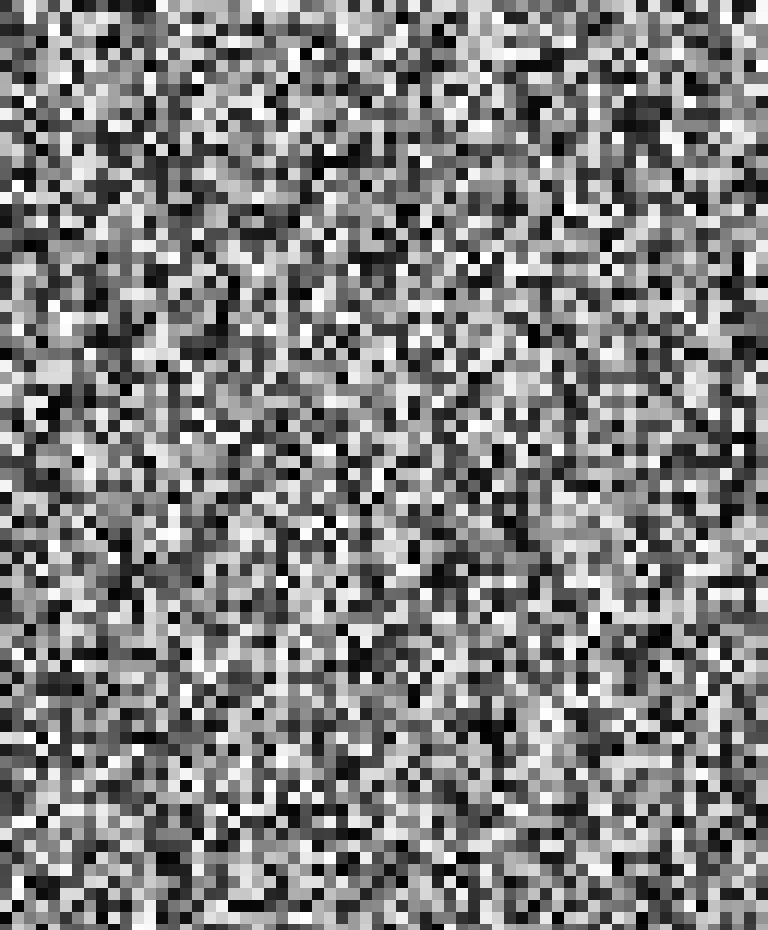
\includegraphics[scale=.9]{img/exp_input_2_cropped.png}
\caption{Generated matrix}
\label{fig:rila}
\end{subfigure}%
~
\begin{subfigure}[t]{0.25\textwidth}
\centering
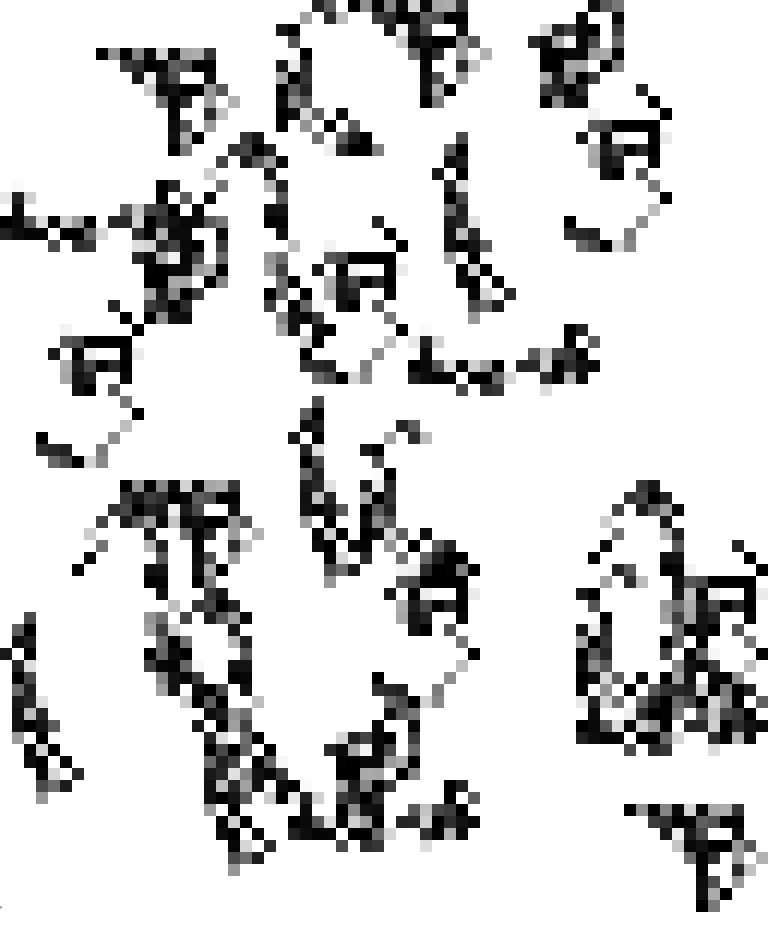
\includegraphics[scale=.9]{img/exp_inputpatterns_2_cropped.png}
\caption{Ground truth}
\label{fig:rilb}
\end{subfigure}%
~
\begin{subfigure}[t]{0.25\textwidth}
\centering
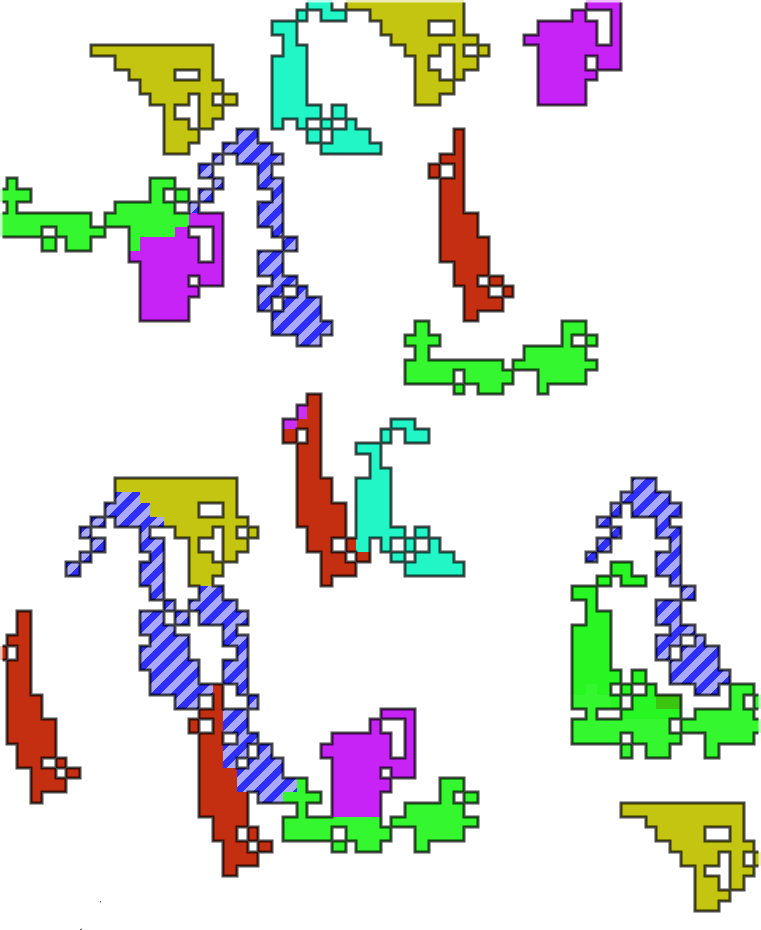
\includegraphics[scale=.9]{img/exp_result_2_cropped.png}
\caption{Found patterns}
\label{fig:rilc}
\end{subfigure}%
~
\begin{subfigure}[t]{0.25\textwidth}
\centering
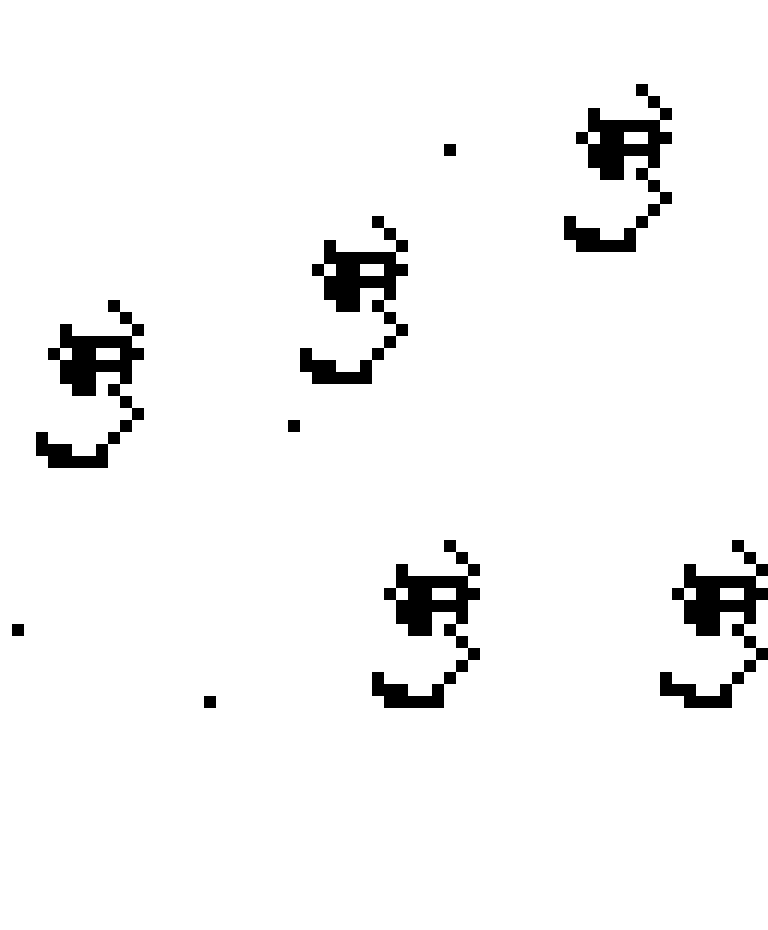
\includegraphics[scale=.9]{img/exp_diff_2_cropped.png}
\caption{Difference}
\label{fig:rild}
\end{subfigure}%
\caption{Synthetic patterns are added to a matrix filled with noise. The difference between the ground truth and the matrix reconstructed by the algorithm is used to compute precision and recall.}
\label{fig:ril}
\end{figure}  

\section{Experiments and Results}

%%
%% The following LaTeX + Gnuplot code generates the two graphs using the gnuplottex package
%% It can be omitted by directly including the pre-baked PDFs as figures
%%
%\begin{comment}

\begin{figure}[t]%
	%\centering%
	\begin{subfigure}[t]{0.5\textwidth}
	%\centering
	\begin{gnuplot}[terminal=epslatex, terminaloptions={color dashed size 6.5cm,4.5cm font "lmodern,8"}]
		set key box bottom left
		set key width 1.0
		set key height 1.0
		set key spacing 1.1
		set key opaque
		set sample 1000
		set xr [0:.7]
		set yr [.3:1]
		set grid xtics lt 0 ls 0
		set grid ytics lt 0 ls 0
		set xlabel 'Signal-to-noise Ratio'
		set ylabel 'Compression'
		#plot "data/256_snr_vs_prec_n10.txt" w l lc 1 lw 1 t "precision",\
		#	 "data/256_snr_vs_recall_n10.txt" w l lc 2 lw 1 t "recall",\
		#	 "data/256_snr_vs_compr_n10.txt" w l lc 3 lw 1 t "ratio"
		plot "data/output_snr_256.txt" using 4:5 w l lc 1 lw 2.5 t "256",\
  			 "data/output_snr_512.txt" using 4:5 w l lc 2 lw 2.5 t "512",\
  			 "data/output_snr_1024.txt" using 4:5 w l lc 3 lw 2.5 t "1024",\
  			 "data/output_snr_2048.txt" using 4:5 w l lc 4 lw 2.5 t "2048"
	\end{gnuplot}}\
	%\caption{The influence of SNR in the ground truth}
	%\label{fig:snr}
	\end{subfigure}%
	%\vspace{-\baselineskip}
	~
	\begin{subfigure}[t]{0.5\textwidth}
	%\centering
	\begin{gnuplot}[terminal=epslatex, terminaloptions={color dashed size 6.5cm,4.5cm font "lmodern,8"}]
		set key box bottom right
		set key width 1.0
		set key height 1.0
		set key spacing 1.1
		set key opaque
		set sample 1000
		set xr [0:50]
		set yr [0:1]
		set grid xtics lt 0 ls 0
		set grid ytics lt 0 ls 0
		set xlabel 'Prevalence per Pattern'
		set ylabel 'Recall' offset 1,0,0
		plot "data/usage_test_128.txt" using 1:8 w l lc 1 lw 2.5 t "128",\
			 "data/usage_test_256.txt" using 1:8 w l lc 2 lw 2.5 t "256",\
			 "data/usage_test_512.txt" using 1:8 w l lc 3 lw 2.5 t "512",\
			 "data/usage_test_1024.txt" using 1:8 w l lc 4 lw 2.5 t "1024"
	\end{gnuplot}
	%\vspace{-\baselineskip}
	%\caption{Prevalence versus recall}
	%\label{fig:usage}
	\end{subfigure}
	%\caption{Qualitative results for increasingly large matrices (sizes are squared). }
	\caption{The influence of SNR in the ground truth (left) and prevalence on recall (right)} 
	\label{fig:plots}
\end{figure}
%\end{comment}

%%
%% End of Gnuplottex section
%%

% Begin of proxy graphs from PDF
\begin{comment}
\begin{figure}[p]%
	\begin{subfigure}[t]{0.5\textwidth}
	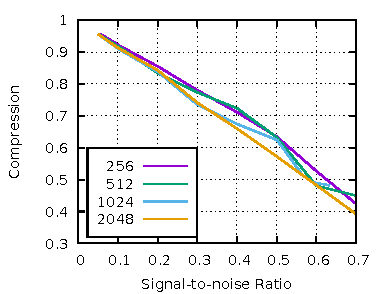
\includegraphics[scale=1]{figures/experiments-gnuplottex-fig1.pdf}
	%\caption{The influence of SNR in the ground truth}
	%\label{fig:snr}

	\end{subfigure}%
	%\vspace{-\baselineskip}
	~
	\begin{subfigure}[t]{0.5\textwidth}
	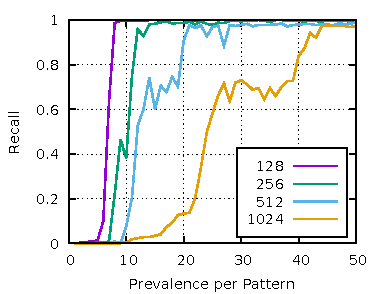
\includegraphics[scale=1]{figures/experiments-gnuplottex-fig2.pdf}
	%\vspace{-\baselineskip}
	%\caption{Prevalence versus recall}
	%\label{fig:usage}
	\end{subfigure}
%	\caption{Qualitative results for increasingly large matrices (sizes are squared).}
	\caption{The influence of SNR in the ground truth (left) and prevalence on recall (right)} 
	\label{fig:plots}
\end{figure}
\end{comment}
% End of proxy graphs


To asses the practical performance of the Vouw algorithm, we will primarily use the synthetic dataset generator Ril that was developed specifically for this purpose. Ril utilizes random walks to populate a matrix with patterns of a given size and prevalence, up to a specified density, while filling the remainder of the matrix with noise. Both the pattern elements and the noise are picked from the same uniform random distribution on the interval $[0;255]$. The \emph{signal-to-noise ratio} (SNR) of the data is defined as the number of pattern elements over the matrix size $MN$. The objective of the resulting experiment is that we try to find all of the signal (the patterns) and none of the noise. Figure \ref{fig:ril} gives an overview of what the generated data looks like, how it is mined and evaluated.

\smallskip \noindent \textbf{Implementation.} %
The implementation\footnote{https://github.com/mickymuis/libvouw} used here, consists of the Vouw algorithm written in vanilla C/C++, a GUI and the synthetic benchmark Ril. 

\smallskip \noindent \textbf{Evaluation.} %
Completely random data (noise) is unlikely to be compressed. The SNR tells us how much noise is present in the data and thus conveniently gives us an upper bound of how much compression could be achieved. We use the ground truth SNR versus the resulting compression ratio as a benchmark to tell us how close we are in finding all the structure in the ground truth. 

Because the compression ratio alone does not tell us the quality of the results, we also compare the ground truth matrix with the compressed result. We use the notion that instances of singleton patterns do not yield any compression and these elements must therefore be noise. Therefore we reconstruct the original matrix from the compressed result, while omitting any singleton patterns. This essentially gives us a matrix of `positives' (signal) and `negatives' (noise). By comparing each element with the corresponding element in the ground truth matrix, traditional figures for \emph{precision} and \emph{recall} can be calculated.

The plots in Figure~\ref{fig:plots} show the influence of input SNR on compression ratio and pattern prevalence on recall, for different matrix sizes. We expect the compression ratio to be close to $1-\mathrm{SNR}$. Patterns with a low prevalence have a lower probability of being `detected' by the algorithm as they are more likely to be accidental/noise. We see that increasing the matrix size also increases this threshold. In Table \ref{table:optimize} we look at the influence of the two improvements upon the baseline algorithm as described in Section \ref{improvements}. In terms of quality, local search can improve the results quite substantial while Best-N notably \emph{lowers} precision. Both improve speed by an order of magnitude, although the improvements given by Best-N are superior. %Another observation is that the baseline algorithm does not scale very favourable with matrix size and that these improvements may be a requisite when mining larger matrices.    

\end{document}


%\section{Discussion}

\documentclass{llncs}
\usepackage[utf8]{inputenc}
\usepackage{verbatim}
\usepackage{multicol}
\usepackage{llncsdoc}
\usepackage{amsmath}
\usepackage{amsfonts}
\usepackage{amssymb}
\usepackage{graphicx}
\usepackage{lmodern}
\usepackage{calc}
\usepackage{enumitem}
\usepackage{algpseudocode}
\usepackage{algorithm}
\usepackage{algorithmicx}

\algsetblockdefx[IfContinue]{IfContinue}{IfContinue}
{0}{0pt}
[0]{}
[1]{\textbf{if} #1 \textbf{continue}}

\algrenewcommand\algorithmicrequire{%
  \makebox[\widthof{\textbf{Output:}}][l]{\textbf{Input:}}}
  
 \algrenewcommand\algorithmicensure{%
  \textbf{Output:}}

\usepackage{color}
\usepackage{gnuplottex}
\usepackage{subcaption}
\usepackage{microtype}
\usepackage[normalem]{ulem}
\captionsetup{compatibility=false}
\usepackage{tikz}
\usetikzlibrary{trees,automata,positioning}
\usepackage{booktabs}
\usepackage{gnuplottex}
\usepackage{xparse}
\usepackage{epstopdf}
% For scaling gnuplottex
\ExplSyntaxOn
\DeclareExpandableDocumentCommand{\convertlen}{ O{cm} m }
 {
  \dim_to_unit:nn { #2 } { 1 #1 } cm
 }
\ExplSyntaxOff

%% For lattice figure
% Set the overall layout of the tree
\tikzstyle{level 1}=[level distance=3.0cm, sibling distance=0.6cm]
\tikzstyle{level 2}=[level distance=3.5cm, sibling distance=0.6cm]
\tikzstyle{level 3}=[level distance=3.5cm, sibling distance=0.6cm]

% Define styles for bags and leafs
\tikzstyle{l1} = [rectangle, text width=5em, text centered]
\tikzstyle{l2} = [rectangle, text width=5em, text centered]
\tikzstyle{l3} = [rectangle, text width=5em, text centered]

% only when using asmthm
%\newtheorem{definition}{Definition}
%\newtheorem{theorem}{Theorem}

\author{Micky Faas \and Matthijs van Leeuwen}
\title{VOUW: Geometric Pattern Mining using the MDL Principle}
\institute{Leiden Institute for Advances Computer Science}
\begin{document}

\section{Conclusions}

We introduced geometric pattern mining, the problem of finding recurring structures in discrete, geometric matrices, or raster-based data. %Compared to most pattern mining problems, it adds a layer of encoding geometric relations of data elements. Furthermore the problem can be split into three classes, of which the first class has been the focus of this paper.
Further, we presented Vouw, a heuristic algorithm for finding sets of geometric patterns that are good descriptions according to the MDL principle. The baseline algorithm is capable of accurately recovering patterns from synthetic data, and the resulting compression ratios are on par with the expectations based on the density of the data. Of the two improvements, especially the local search appears valuable as it improves precision and recall as well as runtime. For the future, we think that extensions to fault-tolerant patterns and clustering have large potential.


%By default, the algorithm has a bottleneck in the candidate search, which can be alleviated by the two demonstrated optimizations of the heuristics. It should also be mentioned that more optimizations on part of the implementation are possible (most notably parallelization), but these are outside the scope of this paper.

%In future work we would like to generalize the formal definition and notation to n-dimensional data. Moreover, the framework can be expanded to cover all three problem classes. For the algorithm, we believe that it can benefit from more refinement on part of the encoding scheme in an effort to lower the threshold of pattern detection in larger matrices. 

\end{document}

\bibliography{bib}{}
\nocite{*}
\bibliographystyle{plain}


\appendix
\documentclass{llncs}
\usepackage[utf8]{inputenc}
\usepackage{verbatim}
\usepackage{multicol}
\usepackage{llncsdoc}
\usepackage{amsmath}
\usepackage{amsfonts}
\usepackage{amssymb}
\usepackage{graphicx}
\usepackage{lmodern}
\usepackage{calc}
\usepackage{enumitem}
\usepackage{algpseudocode}
\usepackage{algorithm}
\usepackage{algorithmicx}

\algsetblockdefx[IfContinue]{IfContinue}{IfContinue}
{0}{0pt}
[0]{}
[1]{\textbf{if} #1 \textbf{continue}}

\algrenewcommand\algorithmicrequire{%
  \makebox[\widthof{\textbf{Output:}}][l]{\textbf{Input:}}}
  
 \algrenewcommand\algorithmicensure{%
  \textbf{Output:}}

\usepackage{color}
\usepackage{gnuplottex}
\usepackage{subcaption}
\usepackage{microtype}
\usepackage[normalem]{ulem}
\captionsetup{compatibility=false}
\usepackage{tikz}
\usetikzlibrary{trees,automata,positioning}
\usepackage{booktabs}
\usepackage{gnuplottex}
\usepackage{xparse}
\usepackage{epstopdf}
% For scaling gnuplottex
\ExplSyntaxOn
\DeclareExpandableDocumentCommand{\convertlen}{ O{cm} m }
 {
  \dim_to_unit:nn { #2 } { 1 #1 } cm
 }
\ExplSyntaxOff

%% For lattice figure
% Set the overall layout of the tree
\tikzstyle{level 1}=[level distance=3.0cm, sibling distance=0.6cm]
\tikzstyle{level 2}=[level distance=3.5cm, sibling distance=0.6cm]
\tikzstyle{level 3}=[level distance=3.5cm, sibling distance=0.6cm]

% Define styles for bags and leafs
\tikzstyle{l1} = [rectangle, text width=5em, text centered]
\tikzstyle{l2} = [rectangle, text width=5em, text centered]
\tikzstyle{l3} = [rectangle, text width=5em, text centered]

% only when using asmthm
%\newtheorem{definition}{Definition}
%\newtheorem{theorem}{Theorem}

\author{Micky Faas \and Matthijs van Leeuwen}
\title{VOUW: Geometric Pattern Mining using the MDL Principle}
\institute{Leiden Institute for Advances Computer Science}
\begin{document}

\section{Appendix}
\label{appendix_a}
\subsection{Prequential Plugin-Code}

To encode the instance matrix we use the \textbf{prequential plug-in code} \cite{grunwaldmdl}. The prequential plug-in code is defined for sequences of one item at a time and updates the probability of each item as it is encoded, such that the probability need not be known in advance. It has the favorable property of being asymptotically equal to the optimal code for large sequences. Say we want to encode all elements ${I}_i \in {I}$, we define:
%\begin{definition}
\begin{align}
P_{plugin}( y_i = {I}_i \mid y^{i-1} ) = \frac{|\{y \in y^{i-1} \mid y = {I}_i\}| + \epsilon }{\sum_{X \in H}|\{y \in y^{i-1} \mid y = X\}| + \epsilon}
\end{align}
%\end{definition}
Here $y_i$ is the i-th element to be encoded and $y^{i-1}$ is the sequence of elements encoded so far. We initialize the base case (no element has been sent yet) with a pseudocount $\epsilon$, which gives $P_{plugin}( y_1 = {I} \mid y^{0} ) = \frac{\epsilon}{\epsilon|H|}$. We pick $\epsilon=0.5$ as it is used generally with good results.

Let us adapt this principle to the problem of encoding patterns. The first step here is to determine the probability that each unique element (instance of a pattern) in ${I}$ occurs. 

%\begin{definition}
\label{usage}
\smallskip \noindent $\triangleright$
\emph{Given a set of instances ${I}$, we define $\mathrm{usage}(X) = |\{ {I}_i \in {I} \mid {I}_i = X\}|.$}
\smallskip
%\end{definition}

From this definition we see that the \textbf{usage} of a pattern is a sum of how often it occurs as an instance. We can use this function to simplify things a little by realizing that we actually know the precise number of instances per pattern on the side of the decoder, but not as the decoder. This information can be used to slightly rephrase Equation \ref{plugin} to be able to encode items in arbitrary order. This produces the length function of the instance matrix ${I}$ as follows\footnote{Here we use the fact that we can interchange sums of logarithms with logarithms of products and that those terms can be moved around freely. Moreover we convert the real-valued product sequences to the Gamma function $\Gamma$, which is the factorial function extended to real and complex numbers such that $\Gamma(n) = (n-1)!$.}:
\begin{align}
\begin{split}
	L_{pp}({I}\mid P_{plugin}) &= \sum^{|{I}|}_{i=1} -\log \frac{|\{y \in y^{i-1} \mid y = {I}_i\}| + \epsilon }{\sum_{X \in H}|\{y \in y^{i-1} \mid y = X\}| + \epsilon}\\
	&= \sum^{|H|}_{X_i \in h} -\log \prod^{\mathrm{usage}(X_i)-1}_{j=0} \frac{j+\epsilon}{\sum^{i-1}_{k=1} U(X_k)+j+\epsilon|H|} \\
	&= -\log \frac{\prod^{X_i\in H} \prod^{\mathrm{usage}(X_i)}_{j=0} j + \epsilon}{\prod^{|{I}|-1}_{j=0} j + \epsilon|H|} \\
	&= -\sum^{|H|}_{X_i \in h} \left[ \log \frac{\Gamma(\mathrm{usage}(X_i)+\epsilon)}{\Gamma(\epsilon)}\right] + \log \frac{\Gamma(|{I}| + \epsilon|H|)}{\Gamma(\epsilon|H|)}
\end{split}
\end{align}

%Lastly, in addition to $L_{\mathbb{N}}$ and $L_{pp}$ we also define the length of the uniform distribution $L_0(n)=log(n)$. That is, when $n$ items have equal probability they all receive a code of equal length $log(n)$.

\subsection{Generating Synthetic Datasets}

This section discusses the synthetic dataset generator Ril, a small utility that produces random matrices and their ground-truths based on several parameters. By testing the output of Vouw on these matrices against the given ground-truth, we can assess both quality and quantity of the patterns discovered by the algorithm. One of the problems with synthetic data generation is that its parameters have a wide range that may or may not have any relation with real use-cases of the algorithm. Moreover, these parameters heavily influence the performance of the algorithm in a way that may not actually be representative, putting an undue bias on the test results. In this section we also explain some of the parameters of Ril and discuss what values we have chosen and why.


\subsubsection{Parameters}

We start by listing all parameters to Ril in Table \ref{table:ril}. Apart from the dimensions, each parameter may require a bit of additional explanation. $|S|$ determines the size of the alphabet or the range of values that each element in the matrix can take. Notice that the actual symbols in $S$ are irrelevant for this purpose; they are discrete and unique values without any semantics. During the experiments we noticed two relations between $|S|$ and the performance of the algorithm: (1) a larger $|S|$ means a larger search space and therefore longer runtime. Especially in the first iterations of the algorithm, more candidates must be considered because more combinations exist in the input. (2) a smaller $|S|$ increases the chance that parts of the noise are identical to (parts of) a pattern. This may lead to false positives (pattern detected in the noise) which could not have been detected by the algorithm (or any algorithm, for that matter).  We have chosen to use a fixed value of $|S|=256$ throughout the experiments. The reason for this is that we wanted to minimize the effect of 'ghost patterns' mentioned above, but also make it 'difficult enough' performance-wise in order to show any potential scaling issues. Moreover, $|S|=256$ mimics regular greyscale images, which we consider a possible use-case in the future. 
  
$P_{\mathrm{noise}}$ and $P_{\mathrm{signal}}$ how likely each symbol in $S$ is to be picked for the noise and signal elements respectively. These distributions can be different from each other, or the same. Statistically it is more difficult to separate signal from noise if $P_{\mathrm{noise}} = P_{\mathrm{signal}}$, which is why we used this scenario exclusively during the experiments. Furthermore we picked both distributions to be uniform, i.e. each symbol has a chance of $\frac{1}{|S|}$ to occur.

\begin{table}
%\centering
\caption{Parameters to Ril and their descriptions.}
\label{table:ril}
\begin{tabular*}{\textwidth}{lll}
\toprule
% & & \multicolumn{4}{c}{Precision/Recall} & \multicolumn{4}{c}{Average time}\\
% \cmidrule(l){3-6} \cmidrule(l){7-10} 
% Size & SNR & None & Local & Best-* & Both & None & Local & Best-* & Both \\
Parameter & Symbol & Description \\
\midrule
Dimensions & $M\times N$ & Width and height of the generated matrix \\
Alphabet & $|S|$ & Number of possible values for each matrix element \\
Pat. size & $[d;D]$ & Range of pattern sizes allowed to occur in the output \\
Pat. occurrence & $[c;C]$ & Patterns occur at least $o$ and at most $O$ times \\
Target SNR & $\mathrm{SNR}_T$ & Actual SNR will be \emph{approximately} this value \\
Distribution & $P_{\mathrm{noise}}, P_{\mathrm{signal}}$ & Random distributions for either noise and signal values \\
Branching fact. & $B$ & Allows hierarchical patterns ($B>0$) or 'flat' patterns \\
& & where no pattern is a subpattern of another ($B=0$) \\
\bottomrule
\end{tabular*}
\end{table}

The \emph{signal-to-noise ratio} (SNR) specifies the ratio of the number of elements belonging to a pattern (signal) versus the number of noise elements. This value is normalized on $[0;1]$. Due to the greedy nature of the synthesizing algorithm, the desired target SNR is approximated rather than exact. This also means that $\mathrm{SNR}=1$ is not possible, but this is hardly relevant with respect to real-world data. We have tested against a variety of SNRs to determine its influence on the algorithm's performance. It appears that low values for SNR generally produce data that is easier to process, because it contains fewer patterns that stand out more clearly against the noise. This may seems somewhat counter-intuitive because high SNRs are associated with cleaner signals. In reality this means that the algorithm is very good at ignoring this particular noise and that it is therefore almost irrelevant in the experiments we did. Further research should therefore probably experiment with different noise types and/or different metrics than SNR.

\subsubsection{Random Patterns}

The pattern generator algorithm in Ril is very simplistic. It uses \emph{random walks} in order to find empty elements to form a pattern, while taking adjacency into account (see the definition of a pattern in Section 3.1).

\subsubsection{Flat and Branching Patterns}



\end{document}

\end{document}